
%\begin{figure}[th]
%	\centering
%	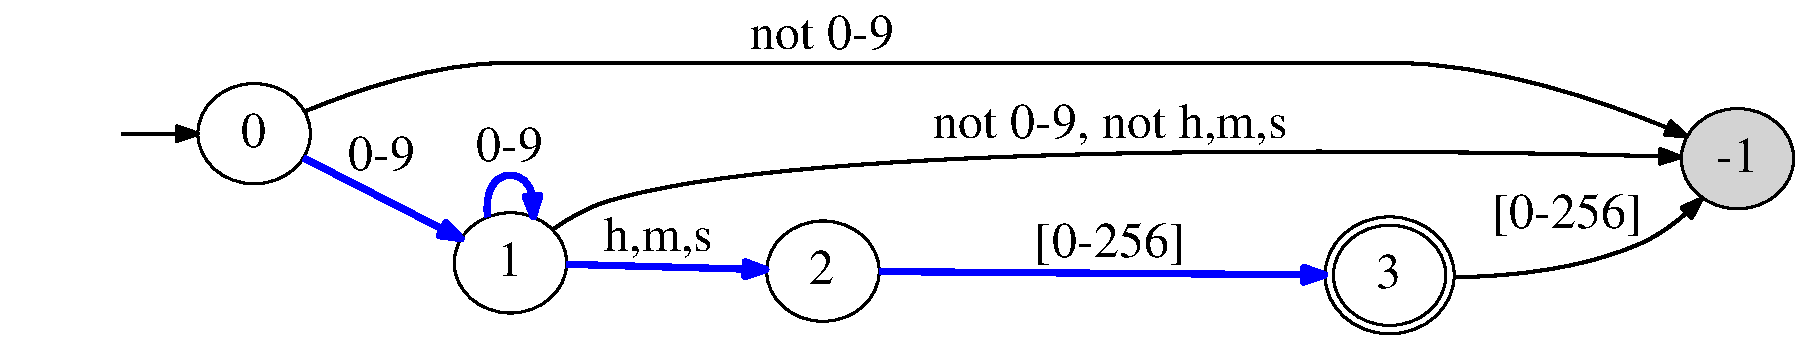
\includegraphics[width=0.5\textwidth]{figures/bugfirstMatch}
%	\vspace{-6pt}
%	\caption{DFA graph generated by RE2~\cite{re2} for the regular expression \texttt{[0-9]+(h|m|s|ms)}. \todo{rename -1 to E}}
%	\label{fig:firstMatch}    
%	\vspace{-6pt}
%\end{figure}~\begin{figure}[th]
%	\centering
%	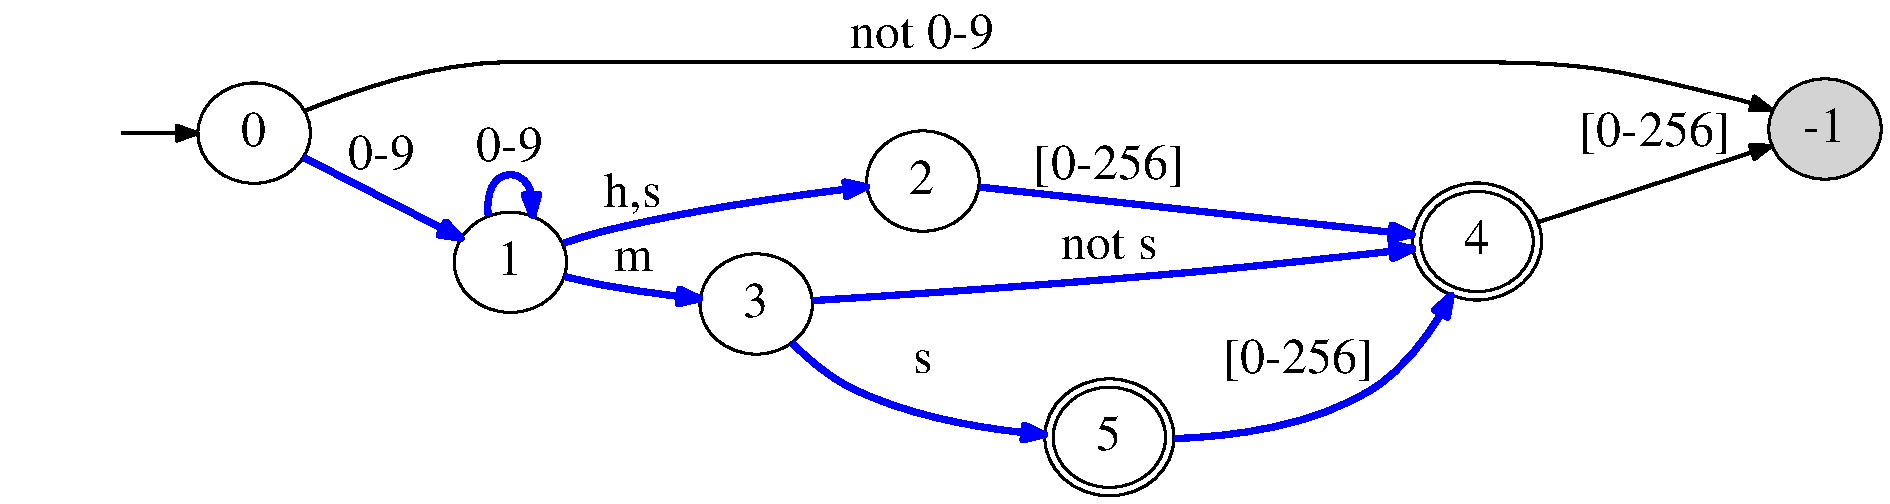
\includegraphics[width=0.5\textwidth]{figures/bugfullMatch}
%	\vspace{-6pt}
%	\caption{DFA graph generated by RE2~\cite{re2} for the regular expressions \texttt{[0-9]+(h|ms|s|m)} and \texttt{[0-9]+(h|m|s|ms)\$}. \todo{rename -1 to E}}
%	\label{fig:fullMatch}    
%	\vspace{-6pt}
%\end{figure}

\section{Background and Motivation}
\label{sec:motive}
%To facilitate a precise description of the work,  we define regular expressions more formally. 
A regular expression is a sequence of characters that defines a search pattern. 
The set of strings matched by the regular expression is a language. 
That is, a regular expression $R$ represents a language $L(R)$ over an alphabet $\Sigma$, where $L(R)$ is a (possibly infinite) set of strings. 
For a given language, there are many regular expressions that can describe it. 
A regular expression can be represented as a string of tokens, a finite state automaton in deterministic (DFA), or a non-deterministic (NFA) form.%, or  a parse tree.


In this work, we explore test coverage metrics over the DFA representing a regular expression. This requires three informal explorations to ensure feasibility and assess the potential impact. 
First, we explore the potential of building DFAs from regular expressions by analyzing regular expressions collected from an existing Python dataset~\cite{chapman2016} and testing them for regularity~\cite{sipser2006introduction}.
Second, we show intuitively how existing coverage metrics are insufficient. 
Third, to motivate the structural coverage metrics, we explore whether faults can lie along untested paths in a DFA. 



\subsection{How Regular are Regular Expressions?}
\label{regularregularexpressions}
Regular expressions in source code can contain non-regular features, such as backreferences. An example is the regular expression \verb!([a-z]+\1)!, which matches a repeated word in a string, such as ``appleapple". Building a DFA is not possible for this since this regular expression is non-regular. For regular expressions in source code that are indeed regular, we can build DFAs and measure coverage based on a test suite. 
Here, we are testing how many of the regular expressions in the wild are truly regular. 

%\adh{These first two paragraphs can be combined and shortened to just say some languages allow non-regular expressions, we need to be able to build a DFA, we're testing how many of the regexes in the wild are truly regular.}
%Regular expression libraries in modern programming languages can contain non-regular features, such as backreferences. 
%This means that a DFA cannot be constructed to represent it. An example is the regular expression \verb!([a-z]+\1)!, which matches repeat words in a string, such as ``appleapple". Building an NFA or DFA to recognize such a pattern is infeasible; it requires a push-down automaton (PDA).  These features may improve the usability of the libraries, but they allow developers to define regular expressions that are not {\em regular} in terms of formal language theory. 
%
%For regular expressions in source code that are indeed regular, we can build DFAs and measure coverage based on a test suite. 
%However, if only a small percentage of regular expressions in the wild are in fact regular, the potential for impact of code coverage metrics that depend on DFAs is limited. 

We explore an existing and publicly available dataset of 13,597 regular expressions scraped from Python projects on GitHub. To test for regularity, we use an empirical approach since the ability to build a DFA from a regular expression implies that it is regular~\cite{sipser2006introduction}. 
Of the 13,597 Python regular expressions, 13,029 (95.9\%) are regular in that we were successful in building DFAs for each using the RE2~\cite{re2} regular expression processing engine. For the remaining 568, we investigated each by hand.  One regular expression was removed because its repetition exceeds the RE2 limits. While it may indeed be regular, to be conservative, we mark it as non-regular. An additional 81 contained comments within the regular expressions, which are unsupported in RE2, so these were also assumed to be non-regular; 128 contained unsupported characters. The remaining 368 were non-regular as they contained backreferences. 

In the end, with nearly 96\% of the regular expressions being regular (as a low estimate), we conclude that most regular expressions found in the wild are regular and thus can be modeled with DFAs. %Thus, the potential for impact was high enough to justify further exploration. 

\subsection{Limitations of Code Coverage}
\label{codecoveragelimits}
In this work, we posit that code coverage metrics~\cite[Chapter~2]{ammann2016introduction}~\cite{zhu1997software,li2009experimental,piwowarski1993coverage} such as statement, branch, and path, are too coarse-grained for regular expressions. Statement coverage requires that the code containing the regular expression is reached, leading to a minimum of one test input for the regular expression. If the regular expression is in a statement where the control flow is dependent on the matching outcome, branch coverage requires that the regular expression have at least two inputs, one that evaluates to true and another that evaluates to false. 
% An alternative is to modify the code related to regular expressions. 

%Regular expression could not be measured in branch coverages, and at the moment there is no tools to measure code coverages of regular expressions. %\footnote{\url{https://stackoverflow.com/questions/3645012/code-coverage-tools-for-regexes}}. 
Consider the following Java code snippet. The \emph{call site} for method {\tt Pattern.matches} is on line~1. The regular expression is \verb!-d|--data!. 

\vspace{-3pt}
\begin{lstlisting}[language=Java]
if(Pattern.matches("-d|--data",strInput)){
	System.out.println("YES");
	...	
}else{
	System.out.println("NO");
	...
}
\end{lstlisting}
\vspace{-3pt}
Statement coverage of the regular expression  requires that line~1 is executed and branch coverage  requires two test inputs, one to cover the {\tt true} branch and one to cover the {\tt false} branch. 
Using coverage metrics based on the DFA representation of the regular expression, on the other hand, 
 would require 1) each branch to be covered, and 2)~each \emph{case} in the regular expression, ``-d" and ``\verb!--!data", to be covered. 
% In fact, such coverage metrics would subsume branch coverage for regular expressions. 
Such metrics measure test coverage of the regular expression's control flow (i.e., the DFA) just like branch coverage measures test coverage of source code's control flow graph.
%While branch coverage builds on the control flow of the source code, DFA coverage builds on the control flow within the regular expression itself.
%The goal is for our definition of regular expression coverage to complement the test coverage metrics and help the automated test generation.

Existing tools and techniques can direct test input generation toward areas of untested paths. % in code, but to date, have not targeted regular expressions. 
One technique among these is symbolic execution~\cite{li2009reggae, king1976symbolic, jpf, klee, Ghosh:2013:JAT:2486788.2486925}, and Rex~\cite{rex} has been developed for symbolic analysis of regular expressions. % but regular expressions are not handled in state-of-the-art tools. 
% However, complex regular expressions in a program may cause the symbolic constraints too complex to solve, thus limiting its use. 
%More lightweight  tools have also been introduced to generate strings for regular expression testing~\cite{rex, kiezun2009hampi, brics, Ghosh:2013:JAT:2486788.2486925}.
However, Rex focuses solely on the matching behavior~\cite{rex}, which limits its ability to cover the false branch in the Java example above. Hampi~\cite{kiezun2009hampi, hampi} and brics~\cite{brics} similarly only generates passing strings. 
%Other tools have the potential to generate both passing and failing strings, such as \todo{which?}. 
%support limited regular expression features~\cite{rex, brics, Ghosh:2013:JAT:2486788.2486925}, traverse the regular expression from the smallest accepted bytes to largest accepted bytes~\cite{brics}, require specified string length~\cite{kiezun2009hampi, brics, Ghosh:2013:JAT:2486788.2486925}, and
While useful, there are no guarantees of structural coverage. 





\subsection{DFA Coverage Example}
\label{sec:coverageexample}
Bug reports related to regular expressions abound. 
 A search for ``regex OR regular expression'' in GitHub yields over 555,000 issues, with 22\% of those still being open. 
 One in particular illustrates how coverage metrics on the DFA could have brought a particular bug to the developer's attention sooner. This bug report\footnote{\url{https://github.com/maven-nar/nar-maven-plugin/issues/228}} describes an issue with the regular expression \verb!\d+\.d+! in the NAR plugin for Maven. 
Figure~\ref{fig:bug} shows the DFA of this regular expression built using RE2~\cite{re2}, and we take this opportunity to describe the DFA notation used throughout this paper\footnote{The regular expression in the bug is triggered by {\tt Matcher.find()} with a ManyMatch DFA. For simplicity, we show the FullMatch DFA, a subgraph of the ManyMatch.}. 

Node~0 is the start-state, indicated by the incoming arrow. 
Nodes with double-circles are accept states, such as Node~4. 
Node~e is the error state, denoting a mismatch. 
The edges are labeled with transitions, often using syntactic sugar for ease of interpretation. 
The edge $\overrightarrow{01}$ is traversed when a digit from \verb!0-9! is read. 
If any other character is read at Node~0, (i.e., \verb!not 0-9!), edge $\overrightarrow{0e}$ is traversed. 
 There is a self-loop on Node~1 for digits \verb!0-9!. 
 If the period character is read from Node~1, then edge $\overrightarrow{12}$ is traversed. 
%If any other character is read (i.e., not `\verb!/!), then edge $\overrightarrow{21}$ is traversed to Node~1. Since Node~1 is an accept state, any other character read from Node~1 reaches the error state, Node~e.

In RE2, when reading an input string, byte~{\tt [256]}, is added as a text-end marker. %, to mark the end of processing. 
For example, the input string ``0.0'' is transformed to the byte stream {\tt [48 46 48 256]}, as {\tt [48]} is the byte for `0', {\tt [46]} is for `.', and {\tt [256]} marks the end of the string. Byte [256] is matched on edges  `\verb![0-256]!', `\verb!not 0-9!',  `\verb!not d!', or `\verb!any except 0-9 and .!'. 

%\todo{replace `[0-256]` in the DFA with `any`; I think it's best not to explain what 256 means at this point}

%\adh{I would delete this paragraph and simply go with the last paragraph: the issue is not testing one of the branches, our approach would have fixed that.  Therefore the problem we are talking about exists in the wild at least sometimes.}
%With the regular expression in Figure~\ref{fig:bug}, input ``/root'' is rejected when it should be accepted, traversing $0 \rightarrow 2 \rightarrow 1 \rightarrow e$. 
%The string ``///''  is accepted should actually be rejected, traversing $0 \rightarrow 2 \rightarrow 2 \rightarrow 2 \rightarrow 1$. This final transition from $2 \rightarrow 1$ occurs because the RE2 tool that built the DFA reads a final byte (byte [256], to be exact) following the last character in the input string to signify the end of processing. The same though would have occurred for ``/root'', except the error state was reached when the first `o' was read, thus no further input characters were processed. 
%and As a result, the urlPattern ``/*'' matches an empty url and does not match the normal url. 
%The traversed path of these three inputs are , , . 

\begin{figure}[t]
	\centering
	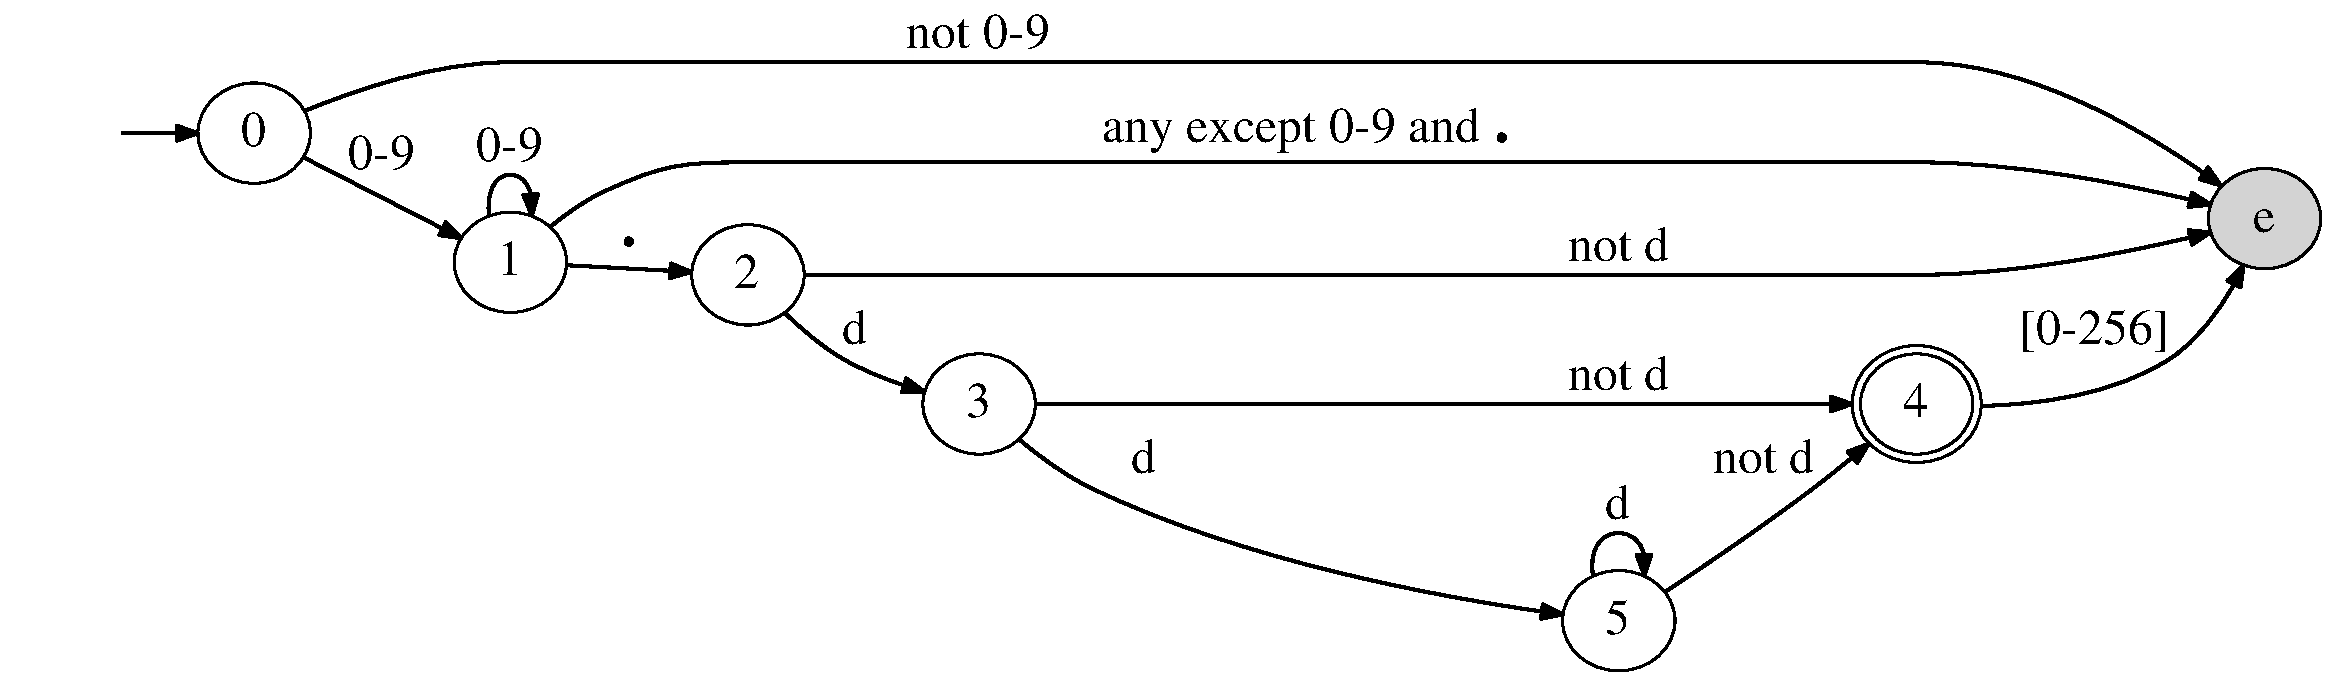
\includegraphics[width=0.48\textwidth]{figures/bug4}
	\vspace{-12pt}
	\caption{Full-match DFA for regular expression: {\tt \textbackslash d+\textbackslash .d+}}
	\label{fig:bug}    
	\vspace{-12pt}
\end{figure}

 The bug report mentions that the regular expression \verb!\d+\.d+! is buggy and the patch adds an escape before the second d, \verb!\d+\.\d+!. The intended behavior is to match input strings with one or more digits, followed by a period, followed by one or more digits.
 
In this work, the structural metrics could reveal this fault. 
With the DFA in Figure~\ref{fig:bug}, when Node~3 is reached, the fault may be revealed. 
Input "0.d" traverses $0 \rightarrow 1 \rightarrow 2 \rightarrow 3 \rightarrow 4$ and ends in an accept state, when it should fail. However, input "0.d3" traverses  $0 \rightarrow 1 \rightarrow 2 \rightarrow 3 \rightarrow 4 \rightarrow e$ and ends in an error state, as expected. 
Covering edge $\overrightarrow{2e}$ may also reveal the fault; input "2.3" traverses $0 \rightarrow 1 \rightarrow 2  \rightarrow e$ and ends in and error state, when it should be accepted.
Requiring coverage of all feasible nodes and edges could have revealed this fault in the regular expression. 

%That is, input "0" traverses $0 \rightarrow 1 \rightarrow e$, the expected behavior, and the fault is not revealed. 
%
%the problematic situation when the empty string ``'' is accepted while should be rejected. 
%The empty string is read as simply {\tt [256]}, traversing $\overrightarrow{01}$ to the accept state. 
%Without testing the empty string, the edge $\overrightarrow{01}$ would be uncovered.
%Presumably, in this case, failure to test the empty string led to a bug report. 
%%According to the bug report, the fix for this regular expression is to replace \verb!/*! with \verb!/.*+!, however, fixing the regular expression is not the goal of the work. 
%The goal of this work is to identify uncovered edges and nodes, such as $\overrightarrow{01}$. 
As with code coverage,  uncovered artifacts alert the programmer to untested behavior. Such coverage information can indicate that a regular expression is not well tested and for some inputs it may not behave as intended, as is the case here.



\iffalse
\begin{figure}[t]
	\centering
	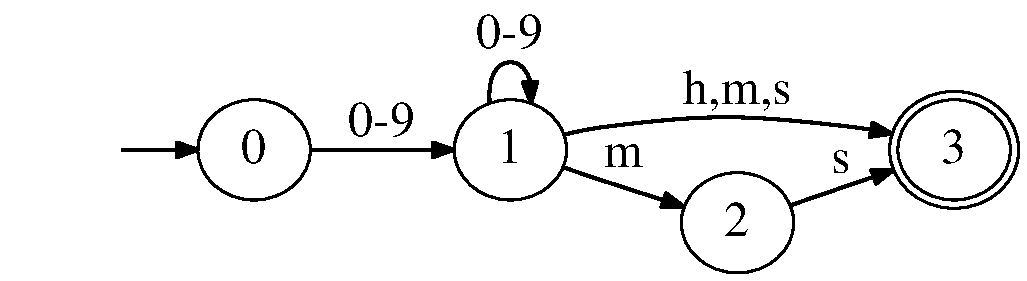
\includegraphics[width=0.35\textwidth]{figures/bugnfa}
	\vspace{-6pt}
	\caption{Finite automata generated for the regular expression \texttt{[0-9]+(h|m|s|ms)}.}
	\label{fig:nfa}    
	\vspace{-6pt}
\end{figure}

\subsection{Are Non-covered Portions of a DFA Problematic?}
The bug reports related to regular expressions abound. One, in particular, illustrates how our proposed coverage metrics could have brought a particular bug to the developer's attention sooner. This bug report\footnote{\url{https://github.com/ebu/ebu-tt-live-toolkit/issues/67}} describes the desired matching behaviors of the regular expression \verb![0-9]+(h|s|m|ms)!. Figure~\ref{fig:nfa} shows finite automata, and we take this opportunity to describe the DFA notation used throughout this paper. 
Node~0 is the start-state, indicated by the incoming arrow. Nodes with double-circles are accept states, such as Node~3. The edges are labeled with transitions, often using syntactic sugar for ease of interpretation. The edge $\overrightarrow{01}$ is traversed when a character in the range of \verb![0-9]! is read. If any other character is read (i.e., \verb!not 0-9!), then the error state (not shown) is reached. There is a self-loop on Node~1 for characters in the range \verb![0-9]!, and an edge $\overrightarrow{13}$ for when \verb!h!, \verb!m!, or \verb!s! is read. 

With the regular expression in Figure~\ref{fig:nfa},  inputs ``9m" and ``9ms" in Python's regular expression matching library are accepted as the extracted string is ``9m", which is correct for the former example, but not the latter. It also accepts ``9mh", when that should be rejected. 
Each of these inputs will traverse nodes $0 \rightarrow 1 \rightarrow 3$, and then stop. 
%The reason lies in the recursive backtracking implementation of Python's {\tt re} engine. 
It interprets the priorities of `h', `s', `m', and ``ms" as the order of their appearance in the regular expression, short-circuiting the evaluation of the entire string. 

%This buggy regular expression could also be explicated by a regular expression engine of DFA implementation. Figure~\ref{fig:firstMatch} shows the DFA graph for the same regular expression. Since the expected matching results for ``9m", ``9ms" and ``9mh" is different, they should cover different nodes and edges of the graph. The matching to ``9m" follows transitions 0$\rightarrow$1$\rightarrow$2$\rightarrow$3, while the latter two follow the same transitions 0$\rightarrow$1$\rightarrow$2$\rightarrow$3$\rightarrow$-1.

The fix for this regular expression is to switch the order of ``ms" and `m' or to change the matching from beginning of inputs\footnote{In Python, {\tt re.match} is defaulted to match from the beginning of inputs, rather than match the entire strong} to from beginning to the end of the inputs. However, fixing the regular expression is not the goal of the work. The goal of this work is to identify edges $\overrightarrow{11}$, $\overrightarrow{12}$, and $\overrightarrow{23}$, and Node~2 as uncovered, alerting the programmer to a possible issue with the regular expression. Such coverage information can indicate when a regular expression is not behaving as intended, as is the case here. The expected path for input ``ms" would be $0 \rightarrow 1 \rightarrow 2 \rightarrow 3$, where the actual path is $0 \rightarrow 1 \rightarrow  3$.

\fi

%In this work, we define and explore coverage metrics for regular expressions. By adopting standard graph-based coverage metrics from the literature, we model regular expressions as DFAs and explore the coverage levels of regular expressions found in GitHub projects. 

%Figure~\ref{fig:fullMatch} shows that ``9m", ``9ms" and ``9mh" have transitions different from each other. ``9m" follows transitions 0$\rightarrow$1$\rightarrow$3$\rightarrow$4; ``9ms" follows transitions 0$\rightarrow$1$\rightarrow$3$\rightarrow$5$\rightarrow$4; and ``9mh" follows transitions 0$\rightarrow$1$\rightarrow$3$\rightarrow$4$\rightarrow$-1.




\section{Test Coverage Metrics}
\label{sec:coverage}
%Traditional test coverage metrics
%% over regular expressions fall short. 
%%Statement coverage just requires that the regular expression be executed. 
%%If the regular expression appears at a branching statement, branch coverage requires that the regular expression be tested with a matching string and a non-matching string~\cite{ammann2016introduction}.
%%However, these metrics 
%ignore much of the complexity within the regular expression. 
We explore fine-grained coverage metrics for regular expressions based on a DFA representation. 
The intuition is that since regular expressions are equivalent to DFAs~\cite{sipser2006introduction}, and 96\% of regular expressions in the wild were found to be regular (Section~\ref{regularregularexpressions}), then graph coverage metrics over the DFA can be used to test the behavior within the regular expression.  
We discuss three levels of coverage: Node Coverage (NC), Edge Coverage (EC), and Edge-Pair Coverage (EPC). These coverage metrics are adopted from graph coverage metrics proposed by Ammann and Offutt~\cite[Chapter 7]{ammann2016introduction}. 
%We explore these coverage metrics in the context of real programs in Section~\ref{sec:rq2}. 
%, and Exit Coverage (EXC)
%\todo{Adopt standard graph notation here, derived from the text, recognizing the text as the source. In standard graph notation, $G = \{V, E\}$. In our work, as in the text, we have special groups of nodes since we are working with DFAs. A graph $G = \{N, N_0, N_f, E\}$ where: $N$ is the set of all nodes, $N_0$ is a set of initial nodes, $N_f$ is a set of final nodes (in our case of DFAs, these are accept nodes), and $E$ is a set of edges}.

%\todo{check whole paper to make sure it's clear that $N_m$ is a set of matching nodes, and if the processing terminates at some $n \in N_m$, then the string is accepted.}
\subsection{Graph Notation} 
For ease of exposition, we expand on the traditional definition of a DFA. In this work, a DFA graph $G = \{N, N_0, N_m, N_e, E\}$ where: $N$ is the set of all nodes, $N_0$ is the initial node, $N_m$ is the final matching/accept node, $N_e$ is the final failing/error node, and $E$ is a set of all edges. 
%\todo{do we need a function to label the edges, like $B(e) = 0-9$ where $e = \overrightarrow{01}$?}
For the DFAs in this work, there is only one initial state, one accept state, and one error state.\footnote{In a FullMatch DFA (see Section~\ref{rq1instrumentation}), there could be several matching nodes, and only one accept. We simplified to use only one accept state.}

The states in a DFA are the nodes $N = \{n_0, n_1, \dots, n_k\}$. 
For any two nodes $n_1$ and $n_2$ such that $\{n_1, n_2\} \subseteq N$, if there is a transition from $n_1$ to $n_2$ in DFA, then the edge $\overrightarrow{n_1n_2} \in E$;  the start and end-state of the path may be the same node, as is the case of self-loops. 
Edge pairs are defined by paths of length two in the DFA.
For example,  if \{$\overrightarrow{n_1n_2}, \overrightarrow{n_2n_3}\} \in E$,  we denote the edge pair as $\overrightarrow{n_1n_2n_3}$.
In the case of self-loops, $\overrightarrow{n_2n_2n_2}$ is also a valid edge-pair. % \in EP$ or $\overrightarrow{n_1n_3n_4} \in EP$. 

Given an input string and a regular expression, the initial node $N_0$ is visited first. Transitions are taken as each character in the string is consumed. The result of the matching process ends in either the accept node $N_m$ or the error node $N_e$. 
In standard DFAs, a traversal can end in any node. However, the DFA generation algorithm used in this work is based on the RE2 tool, which always ends processing in an explicit matching/accept ($N_m$) or error ($N_e$) state.
In this tool, given a regular expression and an input string, the input string is interpreted as a byte stream, with byte {\tt [256]} added to the end to mark the end of the string. Thus, an input string ``2'' would be interpreted as {\tt [50 256]} and the input string ``1001'' would be interpreted as {\tt [49 48 48 49 256]}. 

\looseness +1
As a running example, consider regular expression  $R$ = \verb!\d+! and graph $G$  in Figure ~\ref{fig:static}. %This is a forward-processing DFA, that is, processing of the string starts at the front of the regular e
In $G$, $N~=~\{0, 1, 2, 3, E\}$, $N_0 = 0$, $N_m = 3$, $N_e = e$, 
$E~=~\{\overrightarrow{0e}, \overrightarrow{01}, \overrightarrow{12}, \overrightarrow{13}, \overrightarrow{22}, \overrightarrow{23}, \overrightarrow{3e}\}$, and\\ 
$EP~=~\{\overrightarrow{012}, \overrightarrow{013}, \overrightarrow{122}, \overrightarrow{123},
\overrightarrow{13e}, \overrightarrow{222}, \overrightarrow{223}, \overrightarrow{23e}\}$.  Edges \emph{0-9} cover bytes {\tt [48-57]}, and edges \emph{not 0-9} cover the byte ranges {\tt [0-47][58-256]}; we use the decimal representation to improve clarity. 

%$N_m = \{2, 3\}$ \todo{we need to re-do the graphs AGAIN because $E$ is the set of edges. Let's use a lower-case $e$ for the error state now.}
%, and exits of a regular expression. 


\begin{figure}[t]
	\centering
	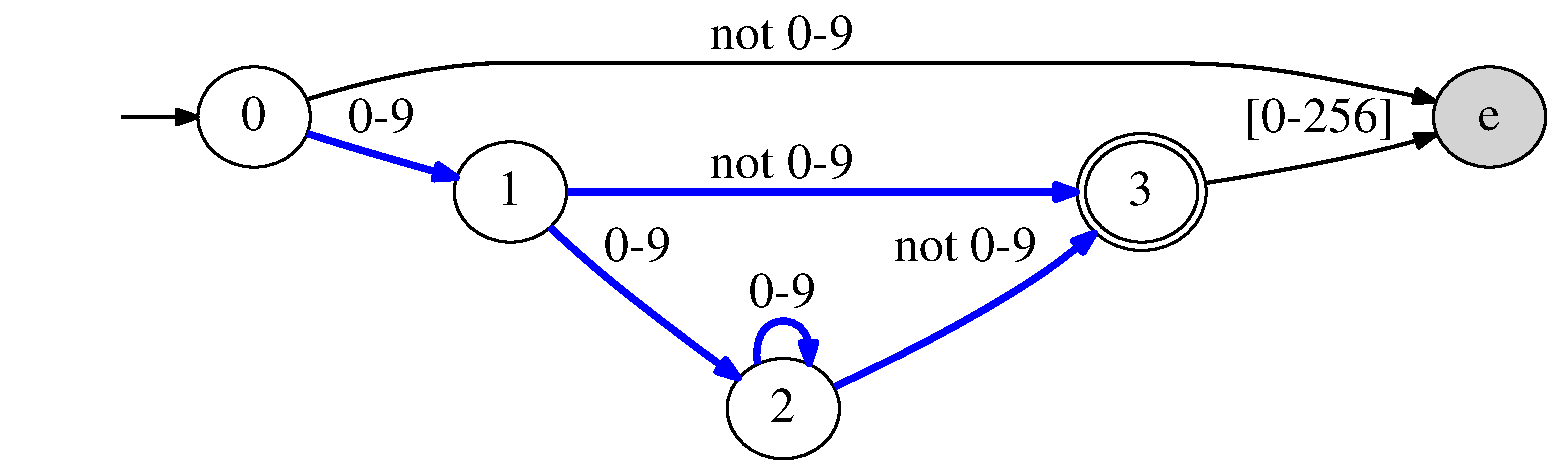
\includegraphics[width=0.45\textwidth]{figures/digits}
	\vspace{-12pt}
	\caption{Full-match DFA from RE2~\cite{re2} for the regular expression {\tt \textbackslash d+}. 
	RE2  interprets every string as a byte stream; the range of bytes is {\tt [0-256]} where {\tt [256]} is added to mark the end of a string. Thus, the input string ``2'' would be represented as {\tt [50 256]} and traverse the following path: $0 \rightarrow 1 \rightarrow 3$. 
	The edges marked \emph{0-9} represent the byte range {\tt [48-57]}; edges \emph{not 0-9} represent the byte ranges {\tt [0-47][58-256]}. }
	%State 2 is the initial state. State 5 is a final matching state. State 1 is a final non-matching state. 
	%\todo{I thought we discussed that non-matching states will all have a single circle, not a double-circle, as the double-circle indicates matching. Please fix. State 1 is a non-matching state with no outgoing edges. This is OK. We don't need to mark it as special.}
%	\todo{is this a first-match DFA?}
%    0-9 are the characters accepted in state transitions. It can also be written as [48-57]. The numbers in square brackets are accepted bytes in decimal in state transitions. [256] indicates there are no more bytes from the input string. The arrows colored blue represent transitions in successful matches.}
	\label{fig:static}    
	\vspace{-6pt}
\end{figure}

%Similar to the DFA in Figure~\ref{fig:bug}, which was used for illustrating our motivation, the DFA in Figure~\ref{fig:static} is a fully specified DFA generated by the RE2 tool~\cite{re2}.
% which interprets every string as a byte stream; the range of bytes is [0-256] where [256] is added to mark the end of a string. Thus, the input string ``2'' would be represented as [50 256] and traverse the following path: $0 \rightarrow 1 \rightarrow 3$. 
%	The edges marked \emph{0-9} represent the byte range [48-57]; edges \emph{not 0-9} represent the byte ranges [0-47][58-256]. 

At this point, we note that this is not the smallest DFA for the regular expression \verb!\d+!.  
%In our work, we build off the RE2~\cite{re2} tool, which generates the DFA shown in Figure~\ref{fig:match1}. 
As the same tool is used for the construction of all the  DFAs, any impact of the DFAs not being minimal  (e.g., extra nodes or edges compared to the minimal representation) is distributed throughout the whole data set and consistent across all experiments. 
%\adh{Does it matter whether the DFAs are minimal (except for performance)?}
While we refer to RE2~\cite{re2} for full details of the DFA construction, though some intuition is provided in Section~\ref{dfamapping}. 



	
%\textbf{Definition of Coverages.} The \emph{node coverage} is the percentage of visited nodes in the static DFA; the \emph{edge coverage} is the percentage of visited edges in the static DFA; the \emph{edge-pair coverage} is the proportion of visited edge pairs in the static DFA; the \emph{exit coverage} is the percentage of visited exits in the static DFA.
\subsection{Coverage Criteria} 
\label{coveragemetrics}
Given a set of strings $S$ and a DFA $G$, for all $n \in N$, we mark $n$ as \emph{covered} if $n$ is visited during the processing of some $s \in S$. Similarly, edges $e \in E$ and edge-pairs $ep \in EP$ are marked as \emph{covered} if they are traversed during the processing of some $s \in S$. The sets of covered nodes, edges, and edge-pairs are denoted $N_{cov}$, $E_{cov}$, and $EP_{cov}$, respectively. 
These sets are aggregated over all $s \in S$. 

As defined in prior work~\cite{ammann2016introduction}, we adopt coverage definitions for node coverage ($NC$), edge coverage ($EC$), and edge-pair coverage ($EPC$) as follows:  

%\footnote{The static DFA is the DFA generated with only the regular expression while the dynamic DFAs are the DFAs generated on-the-fly with the regular expression and its input strings. More details can be found in ~\ref{subsec:cov}}.
%Then the \emph{node coverage} is the percentage of reachable nodes in $G$; the \emph{edge coverage} is the percentage of reachable edges in the $G$; the \emph{edge-pair coverage} is the proportion of reachable edge pairs in $G$. We will omit the edge-pair coverage if there is only one edge in $G$.%; the \emph{exit coverage} is the percentage of reachable exits in $G$.

\begin{definition}[Node Coverage \%]
$NC = \displaystyle{100 \times \frac{\mid N_{cov} \mid}{ \mid N \mid}}$
\end{definition}

\begin{definition}[Edge Coverage \%]
$EC = \displaystyle{100 \times \frac{\mid E_{cov} \mid}{\mid E \mid}}$
\end{definition}

\begin{definition}[Edge-Pair Coverage \%]
$EPC = \displaystyle{100 \times \frac{\mid EP_{cov} \mid}{\mid EP \mid}}$
\end{definition}



%The regular expression `\textbackslash d+'  matches strings consisting only digits. From Figure~\ref{fig:static} we can see that its DFA graph contains five nodes (i.e., 0, 1, 2, 3, and E), seven edges (i.e., $\overrightarrow{0E}$,  $\overrightarrow{01}$,  $\overrightarrow{12}$,  $\overrightarrow{13}$,  $\overrightarrow{22}$,  $\overrightarrow{23}$, and  $\overrightarrow{3E}$), eight edge pairs (i.e., $\overrightarrow{012}$, $\overrightarrow{013}$, $\overrightarrow{122}$, $\overrightarrow{123}$, $\overrightarrow{13E}$, $\overrightarrow{222}$, $\overrightarrow{223}$, and $\overrightarrow{23E}$), one final matching node indicating a match (i.e., 3), and one final non-matching node, representing a non-match (i.e., E).
%\todo{for edge notation, using this notation is more standard. For paths of length 2, I'm not sure if we should use [1, 2, 3] as the book does, or  $\overrightarrow{123}$ for consistency. I'm leaning toward the latter, but for longer paths, we could use the former}.
%2~$\rightarrow$~2, 2~$\rightarrow$~1, 2~$\rightarrow$~3, 3~$\rightarrow$~4, 3~$\rightarrow$~5, 4~$\rightarrow$~4, 4~$\rightarrow$~5, and 5~$\rightarrow$~1), 


%2~$\rightarrow$~2~$\rightarrow$~1, 2~$\rightarrow$~2~$\rightarrow$~2, 2~$\rightarrow$~2~$\rightarrow$~3, 2~$\rightarrow$~3~$\rightarrow$~4, 2~$\rightarrow$~3~$\rightarrow$~5, 3~$\rightarrow$~4~$\rightarrow$~4, 3~$\rightarrow$~4~$\rightarrow$~5, 3~$\rightarrow$~5~$\rightarrow$~1, 4~$\rightarrow$~4~$\rightarrow$~4, 4~$\rightarrow$~4~$\rightarrow$~5, and 4~$\rightarrow$~5~$\rightarrow$~1), one final matching node indicating a match (i.e., 5), and one final non-matching node, representing a non-match (i.e., 1).


To illustrate the coverage levels, consider the graph $G$ for the regular expression \verb!\d+! in Figure~\ref{fig:static} and the string $s_0 = $``2'' with $S~=~\{s_0\}$. 
%Guided by Figure ~\ref{fig:static}, we can describe the process of matching a character `2' to the regular expression `\textbackslash d+'. 
Traversing $G$ visits $0 \rightarrow 1 \rightarrow 3$ (recall that ``2'' is interpreted as the byte stream [50 256]). Node~$3$ is the accept node, which denotes that the regular expression matches the input string (i.e., $s \in L(R)$). 
During the traversal of $G$, nodes \{0, 1, 3\} are visited, meaning that $N_{cov} = \{0, 1, 3\}$, $E_{cov} = \{\overrightarrow{01}, \overrightarrow{13}\}$, and $EP_{cov} = \{\overrightarrow{013}\}$. 
%Therefore, this process covers three visited nodes (i.e., 0, 1, and 3), two visited edges (i.e., $\overrightarrow{01}$, and $\overrightarrow{13}$), and one visited edge pair (i.e., $\overrightarrow{013}$). %This is a successful match. 
The coverage levels for \verb!\d+! by input strings $S = \{s_0\}$ are: $NC$ = 60\%(3/5), $EC$ =  28.6\% (2/7), and $EPC$ =  12.5\% (1/8).% 4) EXC 0\%(0/2).
%2~$\rightarrow$~1, 2~$\rightarrow$~3, and 3~$\rightarrow$~5
%2~$\rightarrow$~3~$\rightarrow$~5



%\todo{check consistency of state vs node}

Next, consider adding the string $s_1$ =``1001'', which is interpreted as the byte stream {\tt [49 48 48 49 256]}. Now, $S = \{s_0, s_1\}$.
Traversing $G$ on $s_1$ traverses the following path: $0 \rightarrow 1 \rightarrow 2 \rightarrow 2 \rightarrow 2 \rightarrow 3$, adding node~$2$ to $N_{cov}$, edges  $\overrightarrow{12}$, $\overrightarrow{22}$, and $\overrightarrow{23}$ to $E_{cov}$, and edge-pairs $\overrightarrow{012}$, $\overrightarrow{122}$, $\overrightarrow{222}$, and $\overrightarrow{223}$ to $EP_{cov}$. 
%Matching the regular expression `\textbackslash d+' with the input `1001' leads to a different process. The DFA transitions from state 2 to state 3 with the byte `1', from state 3 to state 4 with the byte `0', stays in state 4 with the bytes `0' and `1', and from state 4 to matching end state 5 with end indicator byte 256. This DFA graph covers four visited nodes (i.e., 0, 1, 2, and 3), four visited edges (i.e., $\overrightarrow{01}$, $\overrightarrow{12}$, $\overrightarrow{22}$, and $\overrightarrow{23}$), and four visited edge pairs (i.e., $\overrightarrow{012}$, $\overrightarrow{122}$, $\overrightarrow{222}$, and $\overrightarrow{223}$). The edge pair $\overrightarrow{123}$ looks feasible, but it is not visited in this specific process. 
As a result, the coverage levels for the regular expression \verb!\d+! by input strings $S = \{s_0, s_1\}$ are: 
$NC$ = 80\% (4/5), $EC$ = 71.4\% (5/7), and $EP$ = 62.5\% (5/8).
%2~$\rightarrow$~1, 2~$\rightarrow$~3, 3~$\rightarrow$~4, 4~$\rightarrow$~4, and 4~$\rightarrow$~5
%2~$\rightarrow$~3~$\rightarrow$~4, 3~$\rightarrow$~4~$\rightarrow$~4, 3~$\rightarrow$~4~$\rightarrow$~5, 4~$\rightarrow$~4~$\rightarrow$~4, and 4~$\rightarrow$~4~$\rightarrow$~5

As an example of a non-matching string, let $s_2$ = ``u'', which is interpreted as the byte stream {\tt [117 256]}. 
The path traversed in $G$ is $0 \rightarrow e$; after reaching $e$, the processing stops. 
Node $e$ is added to $N_{cov}$, edge $\overrightarrow{0e}$ is added to $E_{cov}$, and there is no change to $EP_{cov}$. 
Considering $S = \{s_0, s_1, s_2\}$, the combined coverage levels are: $NC$ = 100\% (5/5), $EC$ = 85.7\% (6/7), and $EPC$ =  62.5\% (5/8). %4) EXC 50\%(1/2).
%, and one exit (i.e., $\overrightarrow{21}$)
%2~$\rightarrow$~2 and 2~$\rightarrow$~1
%2~$\rightarrow$~2~$\rightarrow$~2, 2~$\rightarrow$~2~$\rightarrow$~1
%2~$\rightarrow$~1
%Because `u' does not belong to the range [48-57], the DFA transitions directly from the start state 2 to the final non-matching state 1. It covers only two nodes (i.e., 1 and 2), one edge (i.e., 2~$\rightarrow$~1), and one exit (i.e., 2~$\rightarrow$~1). The test coverages of the regular expression `\textbackslash d+' by input string `u' are: 1) NC 40\%(2/5); 2) EC 12.5\%(1/8); 3) EPC 0\%(0/11); 4) EXC 50\%(1/2).

For another example of a non-matching string, let $s_3$ = ``100u'', which is interpreted as the byte stream {\tt [49 48 48 117 256]}. 
The path traversed in $G$ is $0 \rightarrow 1 \rightarrow 2 \rightarrow 2 \rightarrow3 \rightarrow e$.
While this input visits all nodes in $G$, $NC = 100\%$ already, so no nodes are added to $N_{cov}$.
 Edge $\overrightarrow{3e}$ is added to $E_{cov}$, edge-pair $\overrightarrow{23e}$ is added to $EP_{cov}$. 
Considering $S = \{s_0, s_1, s_2, s_3\}$, the combined coverage levels are: $NC$ = 100\% (5/5), $EC$ = 100\% (7/7), and $EPC$ =  75\% (6/8). 


For each coverage metric, we compute coverage over the entire set of input strings, \emph{total}, and two subsets: \emph{success}, and \emph{failure}. 
The numbers reported in this section are for the \emph{total} set of input strings, that is, $S = \{s_0, s_1, s_2, s_3\}$. 
After, we split the input strings into those that terminate in an accept state in $N_m$, which we call $S_{succ}$, and those that  terminate in the error state $N_e$, which we call $S_{fail}$. With this example, $S_{succ} = \{s_0, s_1\}$ and $S_{fail} = \{s_2, s_3\}$.

Table~\ref{coverageExample} presents a summary of the coverage levels for each set of input strings. 
%To achieve high EC and EPC, we need to combine both successful matchings $S_{succ}$ and failed matchings $S_{fail}$.
Achieving 100\% for any of the coverage metrics is infeasible for $S_{succ}$ alone because the error state $e$ will never be reached, missing that node and the edges leading to it. 
In this example,  EC for $S_{succ}$ is 71.4\% while EC for $S$ is 100\%.

%The edge-pair coverage for all input strings is only 75\%. To get 100\% coverage of EPC, more inputs are needed. For example, adding string `10' will cover $\overrightarrow{123}$ and adding string `1u' will cover $\overrightarrow{13e}$. 
Achieving 100\% coverage for $EPC$ is the most difficult, but it is possible in this example. 
 The missing edge-pairs are computed by $EP \setminus EP_{cov} = \{\overrightarrow{123}, \overrightarrow{13e}\}$. Two additional input strings can lead to 100\% EPC. Input ``1u'' would be interpreted as the byte stream {\tt [49 117 256]} and traverses the path $0 \rightarrow 1 \rightarrow 3 \rightarrow e$, hence covering $\overrightarrow{13e}$. Input ``11u'' would lead to byte stream {\tt [49 49 117 256]}, traverse the path  $0 \rightarrow 1 \rightarrow 2 \rightarrow  3 \rightarrow e$ and cover $\overrightarrow{123}$. 
%\todo{under what conditions is  impossible to achieve 100\% EPC?}

\begin{table}[tb]
\caption{Coverage of {\tt \textbackslash d+}:  $S = \{``2", ``1001", ``u", ``100u"\}$, \\$S_{succ} = \{``2", ``1001"\}$, and $S_{fail} = \{``u", ``100u"\}$.}
\label{coverageExample}
\vspace{-6pt}
\begin{tabular}{l | r r r}
		& $S$ 	& $S_{succ}$ 	& $S_{fail}$ \\ \hline
$NC$	& 100.0\%	& 80.0\%	 &	100.0\%	\\
$EC$	& 100.0\% & 71.4\% &	85.7\%	\\
$EPC$	& 75.0\%	& 62.5\% &	50.0\%	\\
\hline
\end{tabular}
\vspace{-12pt}
\end{table}

Note that it is possible to have a DFA which is simply two nodes connected by a single edge. Thus, edge pairs may not exist.  For this case, we treat edge-pair coverage as identical to edge coverage. Among the 15,096 regular expressions studied in this work, only two regular expressions have this structure. 

%During regular expression processing, given a string and a regular expression to match against, RE2 uses dynamically-generated DFAs, which are subsets of the static DFA. We compute coverage on this fully static DFA, We refer to RE2 documentation for full details of the construction, 
 

%Another failed matching example is shown by matching the input string `100u' to the regular expression `\textbackslash d+'. The DFA transitions from the initial node 0 to node 2 `100'. Node 2 then transitions to the accept node 3 with the character `u'. In this example, node 3 is not the final node because it continues transitioning to the final error node E with the input end indicator byte 256. Compared to the example of `1001', this process covers one more node (i.e., E), one more edge (i.e., $\overrightarrow{3E}$), same number of edge pairs (i.e., adds $\overrightarrow{23E}$ and misses $\overrightarrow{222}$). The test coverages of the regular expression `\textbackslash d+' by input string `100u' are: 1) NC 100\%(5/5); 2) EC 71.43\%(5/7); 3) EPC 50\%(4/8).
%%5~$\rightarrow$~1
%%4~$\rightarrow$~5~$\rightarrow$~1
%
%The accumulated coverages by input `2' and `1001' are: 1) NC 80\%(4/5); 2) EC 71.43\%(5/7); 3) EPC 62.5\%(5/8). %; 4) EXC 0\%(0/2).
%The accumulated coverages by input `u' and `100u' are: 1) NC 100\%(5/5); 2) EC 85.71\%(6/7); 3) EPC 50\%(4/8). %; 4) EXC 100\%(2/2). 
%If `2', `1001', `u', and `100u' consists of all tested input strings, then the overall test coverages of the regular expression `\textbackslash d+' are: 1) NC 100\%(5/5); 2) EC 100\%(7/7); 3) EP 75\%(6/8). To achieve a 100\% coverage of EPC, more inputs are needed. For example, adding string `10' will cover $\overrightarrow{123}$ and adding string `1u' will cover $\overrightarrow{13E}$.%; 4) EXC 100\%(2/2).




\section{Research Questions}
\label{sec:rq}
To explore the potential of using graph coverage metrics  for regular expressions, we evaluate the following research questions: 
%
%\noindent {\textbf{RQ1:}} {\em What is the impact of under-tested regular expressions?}
%
%\noindent To answer RQ1, we explore publicly available bug reports related to regular expression. By analyzing \todo{number} bug reports and the implicated code, we categorize the impacts of the bug on the software functionality and performance and propose solutions to fix them.

\noindent {\textbf{RQ1:}} {\em How well are regular expressions tested in GitHub?}

\noindent To answer RQ1, we identify 1,225 Java projects that have existing test suites covering the regular expressions. From these, we extract 15,096 regular expressions and 899,804 total test input strings, measuring NC, EC, and EPC for each regular expression. 
To obtain the regular expressions and their corresponding strings which are covered by test cases, we use the Java bytecode manipulation framework Javassist~\cite{javassist} to record the regular expressions when pattern matching methods are triggered by test cases. 
%After eliminating the regular expressions unsupported by RE2~\cite{re2}, we compute coverage based on the strings collected during instrumentation. %We also explore other aspects of regular expressions, such as the percentage of unsupported features, the proportion of pattern mismatching in the total pattern usage, and the replacement of regular expressions with simple string operations.

\noindent {\textbf{RQ2:}}  {\em How well can the regular expression string generation tool Rex  improve the test coverage of regular expressions?}

\noindent Using the regular expressions from RQ1, we generate test strings using Rex~\cite{rex} and calculate the regular expression coverage, comparing it to the coverage of the user-defined test suites from RQ1. 
Using Rex, we generate test suites of three sizes, one to match the size of the user-defined test suites from the GitHub projects, one 5x that size, and one 10x that size. 
%Using Rex, we generate test suites  of three sizes, one to match the size of the user-defined test suites from the GitHub projects so not to bias the results based on test suite size~\cite{coveragetestsuitecorrelation},\adh{the title at least of this reference suggests that coverage does not have an effect on performance, so why would bias occur?} one 5x the size of the user-defined test suite, and one 10x the size of the user-defined test suite, so not to bias against the Rex tool.
%\footnote{The number of accepted strings for some restricted regular expressions is less than 100.}.
%This is because some regular expressions are very restricted and only accept a small number of strings while some other regular expressions are very generic and their accepted strings are innumerable.
%Similar to RQ1, we feed the pairs of regular expressions and their strings into the process of coverage calculation. 
By comparing the coverage statistics we got in RQ2 to those in RQ1, we evaluate the test coverage possibilities through using an automated tool.

%As the research questions operate over different data sets and with different instrumentation, we present each in turn. 

%Because some strings may not increase the coverage of regular expressions at all, we also discuss the least number of strings to achieve the same coverage in RQ3. The results could be a hint for a better method of string compositions in regular expression tools.

%\noindent {\textbf{RQ4:}}  {\em How likely is a regular expression regular?}
%To answer this question, we calculate the percentage of regular expressions based on which we can successfully build the DFA graphs. For the regular expressions on which we cannot successfully build a DFA, they are not regular. Besides the regularity, we also explore the density of DFA graphs and the impacts of different matching types to the construction of DFA graph.

\section{Study}
\label{sec:method}
Applying the coverage metrics defined in Section~\ref{coveragemetrics} to 
regular expressions from the wild requires (1) instrumentation to capture the regular expressions and strings matched against them (Section~\ref{rq1instrumentation}), (2) a tool to measure coverage given a regular expression and a set of strings (Section~\ref{subsec:cov}), and  (3) a large corpus of projects with regular expressions and test suites that execute the regular expressions (Section~\ref{rq1:artifacts}). 
%To achieve (1), we found 1,665 Java projects on GitHub that contain regular expressions and test suites with Maven (Section~\ref{rq1:artifacts}). For (2), we use the Java bytecode manipulation framework Javassist~\cite{javassist} to capture regular expressions and strings matched against them during runtime (Section~\ref{rq1instrumentation}). For (3), we modify the RE2~\cite{re2} regular expression engine to extract the DFA representation and measure coverage (Section~\ref{subsec:cov}). 
To address RQ2, we use the Rex~\cite{rex} tool to generate input strings for the regular expressions in our study (Section~\ref{rq2:artifacts}). 





%The attribute \textit{Projects} represents the number of Java Projects in which the regular expression is used. The attributes of \textit{total inputs}, \textit{unique inputs}, and \textit{projects} indicates the existence of regular expressions used in third-party libraries. They are the noisy data which we will detect and remove from the dataset for coverage analysis. \todo{what does unique inputs mean?} \todo{what does Projects mean?}

\subsection{Instrumentation}
\label{rq1instrumentation}
This section describes our approach to collecting regular expressions from GitHub projects and the strings evaluated against the regular expressions during testing. 

\subsubsection{Instrumented Functions}
\label{sec:instrumentedfunctions}
There are different types of matching between a regular expression and a string. The Java function \emph{Pattern.matches} requires the regular expression to match a string from its beginning to its end; Python's \emph{re.match} requires the regular expression to match a string only from its beginning, not necessarily match to the end of the string; and the C\# function \emph{Regex.Match} requires the regular expression to match only a substring of the input string. These are called \emph{FullMatch}, \emph{FirstMatch}, and \emph{ManyMatch}, respectively. 
%There are two types of matching between a regular expression and a string: \emph{FullMatch} and \emph{ManyMatch}. \emph{FullMatch} requires the entire string to match the regular expression while \emph{ManyMatch} could find all substrings which match the regular expression.
In this work, we consider only \emph{FullMatch} matches and related functions in  Java projects. 
The related functions for FullMatch in Java are:
%\todo{how do you identify if a a full match or many match should be used? fullmatch can be achieved with end-point anchors - do you require the presence of endpoint anchors?}The pattern matching functions we instrumented are:
\begin{itemize}
\item \texttt{java.lang.String.matches(String regex)}
\item \texttt{java.util.regex.Matcher.matches()}
\item \texttt{java.util.regex.Pattern.matches(String regex,\\ CharSequence input)}
%\item \texttt{public boolean String.matches(String regex)}
%\item \texttt{public boolean Matcher.matches()}
%\item \texttt{public static boolean Pattern.matches(String regex, CharSequence input)}
\end{itemize}
\iffalse
\begin{itemize}
\item \texttt{public boolean java.lang.String.matches(String regex)}
\item \texttt{public boolean java.util.regex.Matcher.matches()}
\item \texttt{public static boolean java.util.regex.Pattern.matches(String regex, CharSequence input)}
\end{itemize}
\fi
\noindent In these functions the entire string is required to match the regular expression~\cite{friedl2002mastering}. Thus, a regular expression with end-point anchors (i.e., \verb!^! and \verb!$!) and without are no different. 
%We instrumented these functions and recorded the parameters of pattern and string. 
 
 \subsubsection{Bytecode Manipulation}
 Our instrumentation is built on top of the Java bytecode manipulation framework Javassist~\cite{javassist}, which can dynamically change the class bytecode in the JVM. All the projects are run in jdk1.7. We intercepted FullMatch function invocations in Java. For each invocation, we collect information about the regular expression itself, its location in the code, and any strings matched against it during test suite execution. These strings matched against the regular expression are referred to as the \emph{input strings} or \emph{test inputs} (i.e., $S$ from Section~\ref{coveragemetrics}). %; the set of all input strings matched against a regular expression is called $S$. 
 %Our instrumentation is built on top of the Java bytecode manipulation framework Javassist~\cite{javassist}, which can dynamically change the class bytecode in the JVM. All the projects are run in jdk1.7. First, we built a Java library for the instrumentation that uses {\em jar} files to intercept the invocations of FullMatch functions in Java. For each invocation, we collect information about the regular expression itself, its location in the code, and any strings matched against it during test suite execution. These strings matched against the regular expression are referred to as the \emph{input strings} or \emph{test inputs} (i.e., $S$ from Section~\ref{coveragemetrics}). %; the set of all input strings matched against a regular expression is called $S$. 
% Our instrumentation is built on top of the Java bytecode manipulation framework Javassist~\cite{javassist}, which can dynamically change the class bytecode in the JVM. All the projects are run in jdk1.7. First, we built a Java library for the instrumentation that uses {\em jar} files to intercept the invocations of FullMatch functions in Java. For each invocation, we collect information about the regular expression itself, its location in the code, and any strings matched against it during test suite execution. These strings matched against the regular expression are referred to as the \emph{input strings} \todo{we need to pick a term and be consistent with it}; the set of all strings matched against a regular expression is called $S$. 
%Regular expressions and their input strings are the main information we collected from unit test executions. 


Since a regular expression may also appear in third-party libraries, we use the Java Reflection API to additionally record the caller function stack of the instrumented methods and extract the file name, class name, and method name of their caller methods. 
This allows us to identify when the regular expression being executed is from the system under test and when it is from a third-party library. 
We are dependent on two libraries during the experimentation, {\tt org.junit} and {\tt org.apache.maven}. 
%One drawback of JVM dynamic instrumentation is that it intercepts all method invocation for the instrumented functions, which includes the system under test as well as third-party libraries  imported by these projects (e.g., {\tt org.junit}, {\tt org.apache.maven}). 
Because Maven uses regular expressions to automate unit tests, all recorded regular expressions whose test classes are from package \texttt{org.junit.runner.*} or from package \texttt{org.apache.maven.plugins.*} are treated as regular expressions from third-party libraries and dropped.


%This allows for some data cleanup (Section~\ref{datacleanup}).
%However, because same regular expression may appear in different places of source code and then tested differently in the test suite, we need to calculate their test coverage separately. 
%In order to differentiate between the same regular expression (i.e., that match the same language) but that appear in different code locations, we additionally recorded the caller function invocation of the instrumented methods and extracted the file name, class name, and method name of the caller method. Together with the regular expression, these four pieces of information compose a unique regular expression to calculate its test coverage.

%\begin{figure}[tb]
%\begin{footnotesize}
%\noindent\fbox{%
%\begin{minipage}{0.45\textwidth}
%(1) matches in class: java.util.regex.Matcher[on line number: 559 of file: Matcher.java]\\
%(2) compileRoutePattern in class: kirouter.SinatraRouteParser[on line number: 38 of file: SinatraRouteParser.java]\\
%...\\
%(3) singleParameter in class: KiRouterFilterTest[on line number: 19 of file: KiRouterFilterTest.java]\\
%...\\
%(4) invoke in class: java.lang.reflect.Method[on line number: 606 of file: Method.java]
%...\\
%(5) run in class: org.junit.runners.ParentRunner\$3[on line number: 238 of file: ParentRunner.java]\\
%(6) run in class: org.apache.maven.surefire.junitcore.pc.Scheduler\$1[on line number: 370 of file: Scheduler.java]\\
%...\\
%(7) Matcher matches()---regex: ((:\textbackslash w+)|\textbackslash*)---input: one-name---\#
%\end{minipage}}
%\caption{Instrumentation output for collecting regular expressions and the input strings \todo{can cut for space}}
%\label{instrumentationoutput}
%\end{footnotesize}
%\end{figure}



\subsubsection{Recorded Information}
We illustrate the recorded information for the regular expression \verb!((:\w+)|\*)! and a string ``one-name'' from a project used in our study\footnote{\url{https://github.com/mikko-apo/KiRouter.java}}: %. The following information is retained for analysis: 
%Figure~\ref{instrumentationoutput} shows a snippet of recorded informations for the regular expression \verb!((:\w+)|\*)! and a string ``one-name'' (shown in line (7)) from a project used in our study.\footnote{\url{https://github.com/mikko-apo/KiRouter.java}} Lines (1) to (6) are the caller method information in terms of method name, class name, line number, and file name. For example, line (1) shows the matching is invoked in class {\tt java.util.regex.Matches}, the invoked method is {\tt matches}, and the invocation happens at the line 559 of file {\tt Matcher.java}. Since line (2) is the caller method of the instrumented function, we retain the following location and regular expression information for analysis: 
\begin{itemize}% \itemsep -1pt
\item system under test: {\tt mikko-apo/KiRouter.java}
\item test file: {\tt SinatraRouteParser.java}
\item test class: {\tt kirouter.SinatraRouteParser}
\item test method: {\tt compileRoutePattern}
\item call site: {\tt line 38}
\item regular expression: \verb!((:\w+)|\*)! 
\item input string:``one-name"
\end{itemize}

\noindent In Section~\ref{codecoveragelimits}, the regular expression in the \emph{call site} on line~1 is hard-coded. However, often the regular expression is passed as a variable, allowing multiple regular expressions to be observed during testing at the same call site (i.e., there is a many-to-one relationship between regular expressions and call sites). When this occurs, the recorded information is the same as above, except \emph{regular expression} and \emph{input string} would be different. 
% In the text snippet above, the test file is \textit{KiRouterFilterTest.java} while the matching occurs in file \textit{SinatraRouteParser.java}. 
%\todo{is this correct?}

%Regular expressions which are syntactically same are differentiated by recorded stacks, which consists of a project name, a test method, a test class, a test file, and a regular expression. This is the unit to calculate the coverages for each regular expression. %The unit of our regular expression coverage calculation is a unique regular expression on a recorded stack, consisting a project name, a test method, a test class, a test file, a regular expression, and a set of input strings. 

%However, these frameworks sometimes use regular expressions as well. 
%This muddies the data by including invocations of the targeted Java APIs by code outside the system under test. 
%The matching does not necessarily occur in source code for testing.
%Next, for valid Java Maven Projects in RepoReaper~\cite{repo}, 


%\subsection{Extracting Regular Expressions and Input Strings}
%Given that Maven tests are run in parallel, we forked the JVM and ran the tests separately for each module. In this way, we could collect regular expression information for  modules with passing tests even if other modules' tests failed 
%In this way we dropped 8,496 regular expressions, 1,259 regular expressions which are unique in syntax. 
%The resulting dataset contains 1,256 projects, 15,562 regular expressions, and 14,040 regular expressions which are syntactically unique. 
%Note that the total number of syntactically unique regular expression is larger than 15091 because syntactically regular expressions could appear independently in both stacks of a third-party library and stacks of a GitHub project and thus are countered twice.

%\subsubsection{Limitations}
%To remove the regular expressions used in third-party libraries, we first dropped   \todo{where would thee packages appear? test class? test file? test file?} because these two packages are always used in maven tests. %This left us with 1,665 projects and 24,058 regular expressions.



\subsection{Coverage Analysis}
\label{subsec:cov}
This section details the construction of DFAs for computing coverage. 
Given a regular expression $R$ and a set of input strings $S$, we first build a DFA for $L(R)$  and then track the nodes and edges visited in the DFA during pattern matching with each string $s \in S$. We built our  infrastructure on top of RE2~\cite{re2}, a regular expression engine similar to those used in PCRE, Perl, and other languages.\footnote{Original RE2 at \url{https://github.com/google/re2} and modified code at \url{https://github.com/wangpeipei90/re2}} %Then, we calculate graph coverages according to the description in Section~\ref{sec:coverage}.

\subsubsection{DFA Types.} Given a regular expression and an input string to match, we could build multiple DFAs with different considerations. We could build a static DFA with a regular expression alone or build a DFA on-the-fly (dynamic DFA) considering both a regular expression and an input string. For the same regular expression, different input strings will yield different dynamic DFAs. We can also build a Forward DFA and Backward DFA depending on the direction of scanning the regular expression. These decisions come with various performance tradeoffs during the matching process. 
%Figure~\ref{fig:forwardbackward} shows the differences between a Forward DFA and a Backward DFA for the regular expression \verb!a+b!, which matches one or more {\tt a} followed by exactly one {\tt b}. Its Forward DFA (Figure~\ref{fig:forward}) and Backward DFA (Figure~\ref{fig:backward}) differ in both DFA size and DFA structure. 
For the purpose of our work, we need each DFA to be built consistently regardless of the input string, so we use a static DFA. We chose the forward direction 
%We choose the Forward static DFA for the regular expression and the Forward dynamic DFA for {\em FullMatch} of the regular expression and the input string, since the forward direction is applied in regular expression engines by default and these 
as it seems the most natural for interpretation.

%\subsubsection{DFA Generation} 
\subsubsection{DFA Mapping} 
\label{dfamapping}

%\url{ https://github.com/wangpeipei90/re2}.}. 



%\begin{figure}[t]
%\centering
%  \begin{subfigure}[t]{0.40\textwidth}
%  	\centering
%    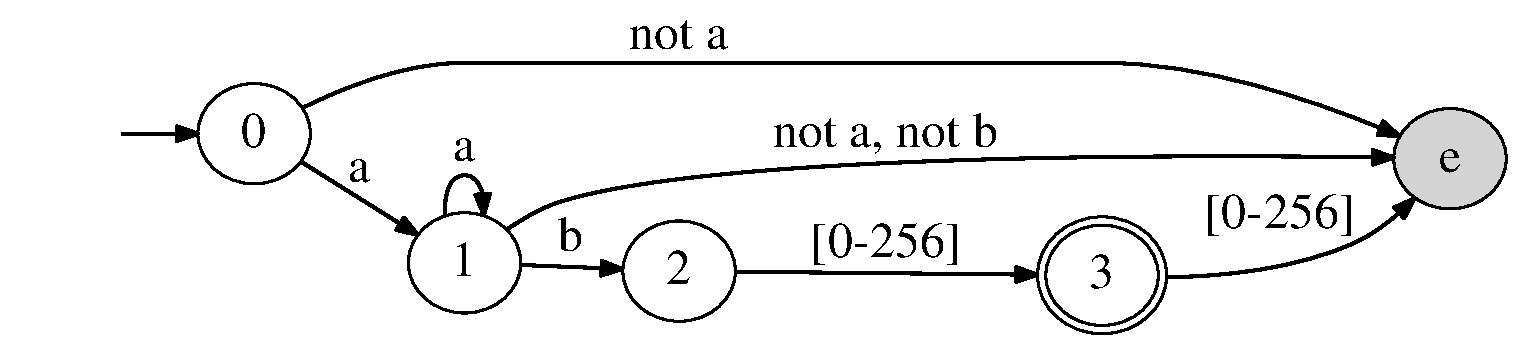
\includegraphics[width=\textwidth]{figures/forwardab}
%    \vspace{-6pt}
%    \caption{Forward FullMatch DFA  }
%    \label{fig:forward}
%  \end{subfigure}
%  
%  \begin{subfigure}[t]{0.4\textwidth}
%  	\centering
%    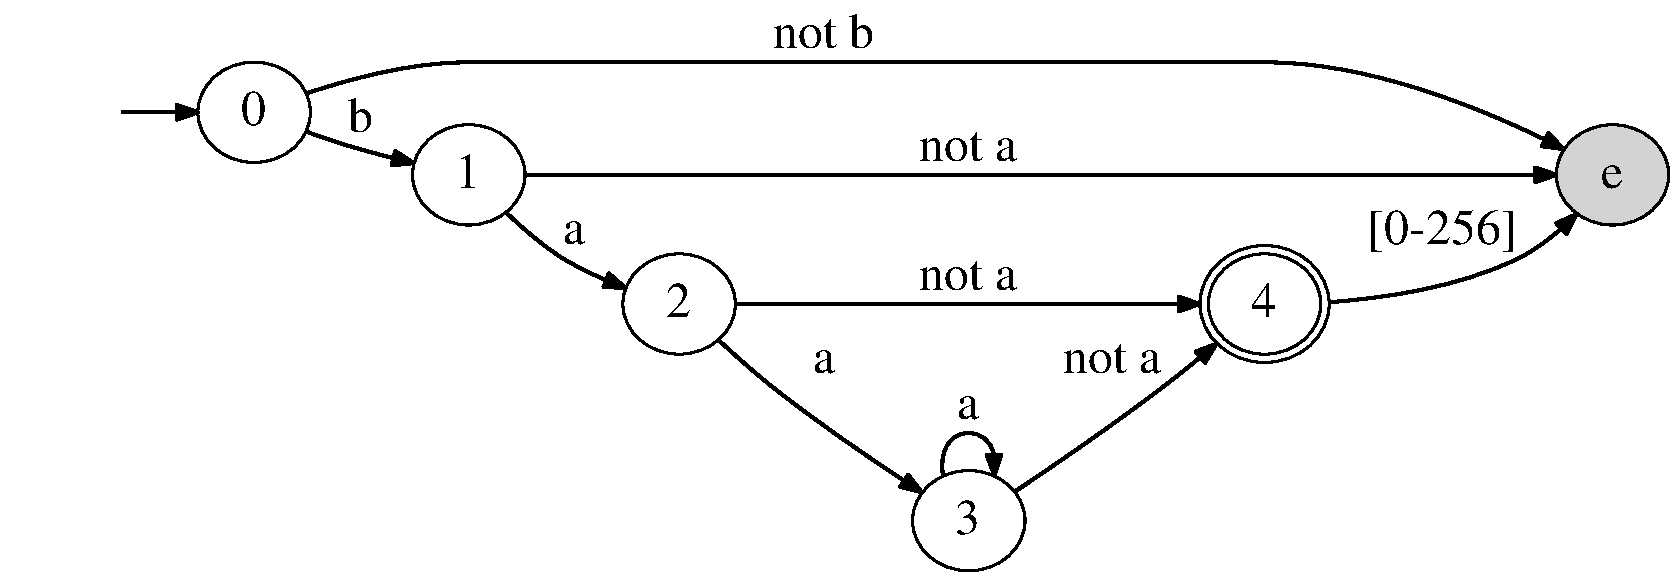
\includegraphics[width=\textwidth]{figures/backwardab}
%    \vspace{-6pt}
%    \caption{Backward FullMatch DFA}
%    \label{fig:backward}
%  \end{subfigure}
%  \vspace{-6pt}
%\caption{Forward DFA and Backward DFA for the same regular expression: {\tt a+b} \todo{can drop for space}}
%\vspace{-6pt}
%\label{fig:forwardbackward}
%\end{figure}

%The process of pattern parsing which expresses the regular expression as the state transition from one state to the next state according to every byte input. It begins with the start state and ends in either a dead state(Ox1) or a match state. By traversing all the transitions and states in this process, we build a graph as the static DFA. Similarly, we build other graphs as dynamic DFAs during the process pattern matching. 






When matching an input string to a regular expression, RE2 builds a dynamic DFA. However, our coverage is computed over a static DFA. This requires mapping to aggregate coverage of a regular expression given multiple input strings. 

For a single regular expression, different input strings often result in different dynamic DFAs. To make matters worse,  these DFAs have inconsistent naming of their states. 
Therefore, to calculate the coverage of a certain regular expression based on the same DFA, these dynamic DFAs have to be mapped to the same static DFA, and then coverage is computed on the static DFA. This is usually straightforward as the dynamic DFA is always an isomorphic subgraph of the static DFA and $N_0$, $N_e$ and $N_m$ are consistently labeled in the static and dynamic DFAs. 
% \todo{is it not always isomorphic?}
%Their start states are equivalent. Each state transition of the dynamic DFA contains one byte input while the equivalent state transition of the static DFA contains a set of byte input. Thus, by traversing the dynamic DFA from the same start state and identifying the arrival states with byte input states, we could make the naming of equivalent states consistent among the static DFA and the dynamic DFAs. 


\begin{figure}[t]
  \begin{subfigure}[t]{0.45\textwidth}
  	\centering
    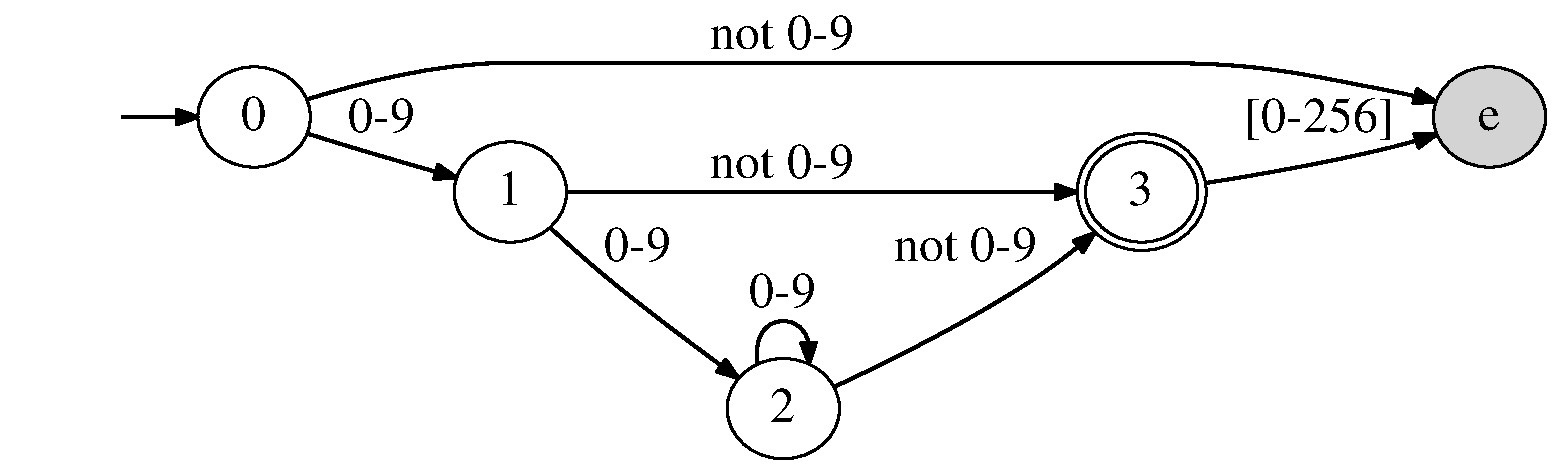
\includegraphics[width=\textwidth]{figures/digitsDFA}
    \vspace{-12pt}
    \caption{Fully specified static DFA for: {\tt \textbackslash d+}}
    \label{fig:staticfull}
  \end{subfigure}

%\vspace{12pt}
%\begin{subfigure}[t]{0.45\textwidth}
%	\centering
%	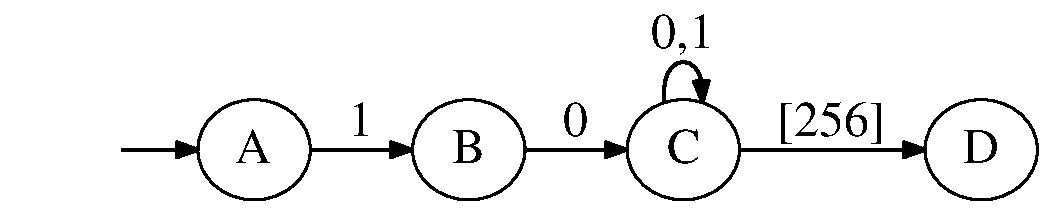
\includegraphics[width=0.6\textwidth]{figures/digits1001mapping2}
%	\vspace{-6pt}
%    \caption{Dynamic DFA prior to mapping for regular expression: {\tt \textbackslash d+} and input: ``1001''}
%	\label{fig:map}    
%%	\vspace{-6pt}
%\end{subfigure}

\vspace{6pt}
  \begin{subfigure}[t]{0.45\textwidth}
  	\centering
    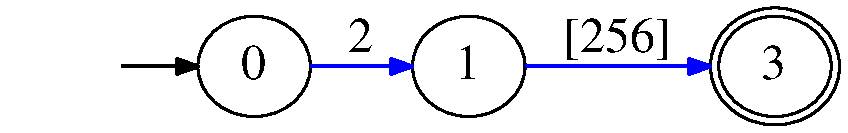
\includegraphics[width=0.5\textwidth]{figures/digits2}
    \vspace{-6pt}
    \caption{Dynamic DFA for regular expression: {\tt \textbackslash d+} and input: ``2''}
    \label{fig:match1}
  \end{subfigure}

\vspace{6pt}

  \begin{subfigure}[t]{0.45\textwidth}
  	\centering
    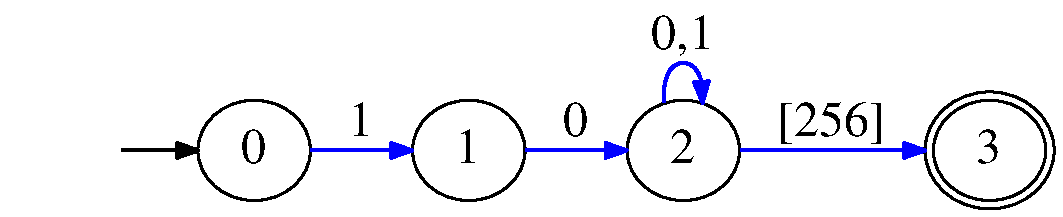
\includegraphics[width=0.6\textwidth]{figures/digits1001}
    \vspace{-6pt}
    \caption{Dynamic DFA for regular expression: {\tt \textbackslash d+} and input: ``1001''}
    \label{fig:match2}
  \end{subfigure}
  
  
  \vspace{12pt}
    \begin{subfigure}[t]{0.45\textwidth}
    \centering
    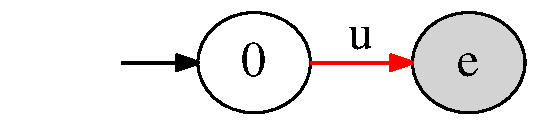
\includegraphics[width=0.3\textwidth]{figures/digitsunew}
    \vspace{-6pt}
    \caption{Dynamic DFA for regular expression: {\tt \textbackslash d+} and input: ``u''}
    \label{fig:mismatch1}
  \end{subfigure}
  
  \vspace{6pt}
  
  \begin{subfigure}[t]{0.45\textwidth}
    \centering
    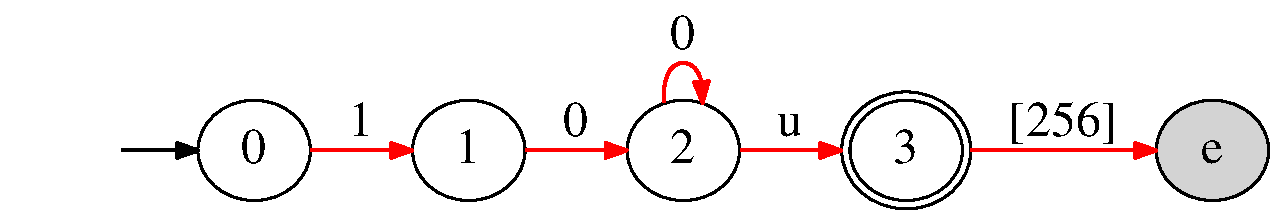
\includegraphics[width=0.7\textwidth]{figures/digits100u}
    \vspace{-6pt}
    \caption{Dynamic DFA for regular expression: {\tt \textbackslash d+} and input: ``100u''}
    \label{fig:mismatch2}
  \end{subfigure}
\vspace{-6pt}
\caption{Visited DFA subgraphs for the regular expression {\tt `\textbackslash d+'}.  For each figure, $N_0$ is the initial node 0, $N_m$ is the accept node 3, $N_e$ is the error node e. 
%State 2 is the initial state. State 5 is a final matching state. State 1 is a final non-matching state. 
The arrows colored blue represent transitions in successful matches. The arrows colored red represent transitions in failed matches. %\todo{is there any reason to have these colored edges? If no, make them all black. It doesn't seem to add value.}
%Each ellipse in the graph represents one state of the DFA. The ellipse labeled `2' with an incoming arrow is the start state of DFA. The ellipse with double circles is the end states of DFA. The unfilled double-circled ellipses are matching end state of DFA, which implies a successful match between the regular expression and the string. The gray double-circled ellipse with double circles labeled `1' is the error end state, which implies a failure in matching the string to regular expression. A state with an input of a byte transitions to another state. 
    The characters without square brackets are the literal characters in state transitions. For example, `u' prompts the transition from Node 0 to Node e. {\tt [256]} implies that there are no more bytes from the input string.}
\vspace{-12pt}
\label{fig:dfas}
\end{figure}

Consider the regular expression \verb!\d+! and $S = \{s_0, s_1, s_2, s_3\}$ from Section~\ref{coveragemetrics} where $s_0$ = ``2'', $s_1$ = ``1001'', $s_2$ = ``u'', and $s_3$ = ``100u''. Figure~\ref{fig:staticfull} shows the static forward DFA. %From this point, all DFAs are assumed to be forward. 
The dynamic DFAs corresponding to these four inputs are shown in Figure~\ref{fig:match1}, Figure~\ref{fig:match2}, Figure~\ref{fig:mismatch1}, and Figure~\ref{fig:mismatch2}, respectively. Blue arrows are used to identify the visited edges in the dynamic DFAs when the input string is a match. Red edges are used to identify the visited edges when the input string is not a match. 
% after mapping to its static DFA, excepting Figure~\ref{fig:map}, which shows the original dynamic DFA for \verb!\d+! and $s_3$ \emph{prior} to mapping onto the static DFA. 
Note that in Figure~\ref{fig:dfas}, for simplicity, we have already mapped and renamed the nodes in the dynamic DFAs according to the static DFA. % in Figure~\ref{fig:staticfull}
%In reality, there is a step in which each of the nodes in the dynamic DFAs is mapped onto the static DFA. This mapping process is straightforward as $N_0$, $N_e$ and $N_m$ are consistently labeled in the static and dynamic DFAs. %\todo{Peipei, is this last sentence correct?}

% we temporarily denote them as \emph{A,B,C,D}. The traversal of this DFA is $A \rightarrow B \rightarrow C \rightarrow C \rightarrow C \rightarrow D$. Consider the static DFA in Figure~\ref{fig:staticfull} (equivalent to Figure~\ref{fig:static}, but repeated here for easier reading). 
%The initial state is straightforward to map, and $A \mapsto 0$. 
%The transition in the dynamic DFA is along edge $\overline{AB}$ with input $1$. 
%The same input in the static DFA traverses edge $\overline{01}$, and so $B \mapsto 1$. 
%Similarly, $C \mapsto 2$.
%Since the final state D is not the error state, state D is regarded as the final accept state and  $D \mapsto 3$. The results of mapping Figure~\ref{fig:map} is shown in Figure~\ref{fig:match2}.%\todo{why is ((2)) an accept state if it's impossible to accept anything from it (that is, there is no in-arrow of byte 256)?}




\subsubsection{RE2 Limitations and Modifications}
\label{dfageneration}
% There are some other modifications of the RE2 source code so that the DFAs could be publicly visible and accessible to operate. 
We enlarged the default memory size of a cached DFA so that it could accommodate large DFA graphs. Due to Linux environment limitations, string length is limited to 131,072 and null type is not allowed.
%We changed the default memory size of a cached DFA from 1MB to 256MB so that it could accommodate large DFA graphs. 
%However, due to the maximum length of a single argument in Linux environment (131,072), input strings longer than 131,071 characters are dropped from generating dynamic DFAs. Null byte \verb!\x00! is not acceptable as an argument and input strings containing \verb!\x00! are dropped as well. 
%However, due to the string length limitation of bash scripts \todo{huh? why does a bash script matter? is Re2 dependent on bash scripts? this limitation isn't straightforward as described}, input strings longer than 131,071 characters are dropped from generating dynamic DFAs. 
% Null byte \verb!\x00! is not acceptable in bash scripts and input strings containing \verb!\x00! are dropped as well. 
 These situations are rare, impacting  $<1$\% of the collected regular expressions (see Section~\ref{rq1:artifacts}). 



\subsubsection{Coverage Calculation} 
With the consistent naming between a static DFA and a dynamic DFA, all nodes, edges, and edge pairs in the latter are regarded as visited nodes, edges, and edge pairs of the former. 
That is, a node only appears in a dynamic DFA when it is visited during matching; these can be thought of as \emph{just-in-time} DFA constructions in the context of a string to match. 
The coverage metrics from Section~\ref{coveragemetrics} are computed over the static DFAs, aggregating over all input strings observed during testing. 



%For regular expressions and tool-generated strings, all strings are matched to their corresponding regular expressions successfully. We report the test coverages of nodes, edges, and edge pairs for each regular expression. However, for data collected in GitHub projects, some input strings could fail to match their regular expression.s. As a result, we report the test coverages differently: 

%As there exists both successful matches and failed matches, we report the test coverage in three aspects: 1) the test coverages of nodes, edges, and edge pairs for the regular expression given successfully matched input strings; 2) the test coverages of exits, nodes, edges, and edge pairs for the regular expression given failed matched input strings; 3) the test coverages of nodes, edges, and edge pairs for the regular expression given all input strings.



%As explained in Section~\ref{coveragemetrics}, the coverage metrics are computed over the total set of input strings $S$ as well as over the set of input strings that lead to an accept state, $S_{succ}$ and those that lead to a failure state, $S_{fail}$. 

%\subsection{Existing Tools Analysis (RQ2)}

%We first calculated the coverages with same number of unique inputs as these in GitHub project, then we calculated again with all the unique inputs we got from Rex.


\subsection{Artifacts for RQ1}
\label{rq1:artifacts}
%This section illustrates the artifacts used in our analysis related to test coverages of regular expressions. We show first how we collect regular expression.related bugs, then describe the repository to analyze test coverage in community, and finally present the dataset used to measure the effectiveness of regular expression tools.
RepoReaper~\cite{reporeaper} provides a curated list of GitHub projects with the ability to sort based on project properties, such as the availability of test suites, which is a pre-requisite for our study. 
We focused on Java projects due to its popularity on GitHub and the availability of a bytecode analysis framework for instrumentation. 

%We extracted regular expressions and matching strings from GitHub Java projects. 

\subsubsection{Project Selection}
In December 2017, we selected the 136,196 Java projects whose unit test ratio reported in RepoReaper is greater than zero. %that have unit tests from RepoReaper. 
Because the density of regular expressions in projects tends to be low, we automated project builds and test suite execution in order to collect sufficient data. As such, we require all projects we analyze to use 
\textit{maven} and \textit{junit} to automatically run unit tests. 
We identified 13,637 Java Maven projects that used Java pattern matchings functions mentioned in Section~\ref{rq1instrumentation}. From those, we selected the ones that could be successfully compiled and tested in Maven, leaving 5,691  projects on which we attempted to collect coverage information. 
%Due to the environment dependency limits and execution time limits, we could not compile and run unit tests for all projects listed in RepoReaper. 
%To achieve a regular expression corpus similar in size to previous work using Python~\cite{chapman2016}, we set a goal of finding 15,000 unique regular expressions.  



%\begin{table}[tb]
%%\centering
%\caption{Description of dataset changes.}
%\label{data:change}
%\begin{small}
%%\resizebox{0.5\textwidth}{!}{%
%%\begin{tabular}{lllllllll}
%\begin{tabular}{p{2.5cm}
%>{\raggedleft\arraybackslash}p{0.6cm}
%>{\raggedleft\arraybackslash}p{1.6cm}
%>{\raggedleft\arraybackslash}p{2.6cm}}
%\hline
%Operation & Projects & Regular Exp. & Unique Regular Exp.\\
%\hline
%Instrumentation 	& 1,665  & 24,058 & 15,091 \\
%Regular Exp. Removal & 1,256 & 15,562  & 14,040  \\  
%Static DFA 			& 1,225  & 15,105  & 13,638 \\
%Dynamic DFA 		& 1,225  & 15,096  & 13,632\\ 
%Multi-inputs		& 1,014	 & 8,778  & 7,947 \\
%Rex(ASCII)		    & 1,057	 & 12,184 & 10,946\\
%Rex(Unicode)		& 1,057	 & 12,181 & 10,943\\
%\hline
%\end{tabular}
%%}
%\end{small}
%%
%%\vspace{5pt}
%%
%%\vspace{-12pt}
%\end{table}


\subsubsection{Regular Expression and Test Input Collection}
To collect the input strings for each regular expression, we instrumented each project and executed the test suites. 
We changed the configurations of the plugin \emph{maven-surefire-plugin}  by adding {\em -javaagent} argument to {\em argLine} so that when Maven forks a VM to run the unit tests the VM can load the instrumentation library. 
Each project module that runs tests executes in different VMs and the information is recorded in different files. {\em testFailureIgnore} is configured to {\em true} so that one test failure does not affect the other tests, allowing us to record as many regular expressions in the project as possible.
%In collecting the test inputs for each regular expression, we changed the configurations of the plugin \emph{maven-surefire-plugin}  by adding {\em -javaagent} argument to {\em argLine} so that when Maven forks a VM to run the unit tests the VM can load the instrumentation library. 
%Each project module that runs tests executes in different VMs and the information is recorded in different files. {\em testFailureIgnore} is configured to {\em true} so that one test failure does not affect the other tests, allowing us to record as many regular expressions in the project as possible. %\todo{This information seems important and I don't know where to put it}

Of the 5,691 projects with Maven, test suites, and pattern matching functions, 1,665 projects contained 24,058 regular expressions executed by test suites. The remaining projects contained regular expressions \emph{not} executed by the test suites, and thus could not be instrumented. 



\subsubsection{Filtering Out Third-Party Regular Expressions}
%We regard the remaining regular expressions being used in method invocations of third-party libraries are outliers. We detect them using the rule of IQR(InterQuartile Range)~\footnote{\url{https://en.wikipedia.org/wiki/Interquartile_range}}. We calculate the total amount of matching invocations for all regular expression. If the first and third quartiles are denoted by $Q1$ and $Q3$, then $IQR=Q3-Q1$. For a regular expression $r$, its total invocations is denoted $t(r)$. If $t(r)>Q3+1.5*IQR$, then $r$ will be dropped as a regular expression from third-party libraries. 
%The remaining regular expressions being used in method invocations of third-party libraries are identified by their proportions in the whole data set. A regular expression is dropped if it is used widely across different projects. We set the threshold to 10\% of all projects. 
%\todo{is the following still relevant?} If a regular expression is matched to a large number of different inputs (i.e, above the 90 percentile of them from 15091 regular expressions), we drop it as well. \todo{if the unique inputs that it is used frequently to match is above the 90 percentile of all regular expressions -- reword please. I don't follow.}. 
FullMatch invocations from Maven and JUnit have been removed already at this point, but other third-party libraries also use regular expressions. 
We can detect this by looking for syntactically identical regular expressions with invocations on the same file, same class, same method, but in different GitHub projects. 
%We assume that there are no such projects which call the same third-party function and pass along the same regular expression as the argument of that function. 
%Therefore, we detect third-party library invocations by identifying pairs of identical regular expressions and stack information in different projects.
If the number of projects is larger than one, then it is regarded as a third-party regular expression, and all records related to the same stack information are dropped. 
A limitation of this approach is that we miss some third-party invocations that are only present in a single project. Given the large number of projects analyzed, the impact of this is likely to be small. 
 
 We identified 8,496 regular expressions as coming from third-party libraries. %, 1,259 of which were syntactically unique. 
 The resulting dataset contains 1,256 projects and 15,562 regular expressions, 14,040 of which are syntactically unique. %The overall full matches in the 1,256 projects are 1,8514. 
%In this way we dropped 8,496 regular expressions. %, 1,259 of which were syntactically unique. 
%The resulting dataset contains 1,256 projects and 15,562 regular expressions, 14,040 of which are syntactically unique. The overall full matches in the 1,256 projects are 1,8514.

%A limitation of this approach is that we miss some third-party invocations that are only present in a single project. \todo{any mitigation for this? Perhaps move this to threats to validity}

\begin{table}[tb]
%\centering
\caption{Description of 1,225 Java Projects Analyzed. All numbers are rounded to nearest integer except the test ratio and KLOC.}
\label{regex:distriprojects}
\vspace{-6pt}
\begin{small}
%\resizebox{0.5\textwidth}{!}{%
%\begin{tabular}{lllllllll}
%\begin{tabular}{p{3.2cm}@{}
%>{\raggedleft\arraybackslash}p{0.5cm}
%>{\raggedleft\arraybackslash}p{0.5cm}
%>{\raggedleft\arraybackslash}p{0.5cm}
%>{\raggedleft\arraybackslash}p{0.5cm}
%>{\raggedleft\arraybackslash}p{0.5cm}
%>{\raggedleft\arraybackslash}p{0.6cm}}
\begin{tabular}{p{2.4cm}@{}r r r r r r}
\hline
Attributes & mean & 25\% & 50\% & 75\% & 90\% & 99\%  \\
\hline
%Regular exp. & 14 & 2    & 5     & 13    & 25    & 90 \\
%Stars& 40 & 0    & 1     & 4    & 26    & 771 \\
%Test ratio & 0.230 & 0.080 & 0.196 & 0.340 & 0.473 & 0.728\\ 
%kLOC & 63 & 2 & 8 & 32 & 119 & 910 \\ 
%Size(KB) & 19530 & 318 & 1347 & 9118 & 41408 & 273233 \\ 
Tested Regular exp. & 12 & 1    & 3     & 7    & 18   & 99 \\
%Stars& 16 & 0 & 1 & 3 & 19 & 356 \\
Stars& 35 & 0 & 1 & 5 & 30 & 833 \\
Test ratio & 0.238 & 0.096 & 0.210 & 0.346 & 0.482 & 0.691\\ 
%kLOC & 55,382 & 2,046 & 6,743 & 25,101 & 86,718 & 951,007 \\ 
KLOC & 55.4 & 2.0 & 6.7 & 25.1 & 86.7 & 951.0 \\ 
Size (KB) & 19,062 & 286 & 1,079 & 6,449 & 33,163 & 249,915 \\ 
\hline
\hline
Call sites 		  & 15 & 2 & 4 & 10 & 31 & 211 \\
Tested call sites & 3 & 1 & 2 & 3 & 6 & 20 \\
%\hline
%Regular exp./call site & 1 & 0 & 0 & 0 & 1 & 8 \\
Reg. exp./tested site & 5 & 1 & 1 & 2 & 5 & 38 \\
\hline
\end{tabular}
%}
\end{small}
\vspace{-6pt}
\end{table}


\begin{table}[tb]
%\centering
\caption{Description of 15,096 regular expressions analyzed for RQ1. All numbers are rounded to nearest integer}% \todo{shouldn't this be 15,096?}}
\label{regex:distriregex}
\vspace{-6pt}
\begin{small}
%\resizebox{0.5\textwidth}{!}{%
%\begin{tabular}{lllllllll}
\begin{tabular}{p{2.2cm}
>{\raggedleft\arraybackslash}p{0.6cm}
>{\raggedleft\arraybackslash}p{0.6cm}
>{\raggedleft\arraybackslash}p{0.5cm}
>{\raggedleft\arraybackslash}p{0.6cm}
>{\raggedleft\arraybackslash}p{0.6cm}
>{\raggedleft\arraybackslash}p{0.7cm}}
\hline
Attributes & mean & 25\% & 50\% & 75\% & 90\% & 99\%  \\
\hline
Nodes ($\lvert N \rvert$) & 144 & 12  & 28   & 70   & 324  & 939   \\
Edges ($\lvert E \rvert$) & 565 & 24  & 75   & 212  & 938 & 2,813  \\  
Edge pairs ($\lvert EP \rvert$) & 2,115 & 25   & 99   & 414  & 1,647 & 16,850 \\
Regular exp. len. & 31  & 13 & 18 & 39 & 67 & 161 \\
\# Input strings ($\lvert S \rvert$) & 60 & 1    & 2    & 7  & 27  & 662  \\ 
Input string len. & 125 & 9 & 17 & 63 & 318 & 948 \\ 
%Input length dev. & 115.76 & 0.00 & 2.12 & 15.45 & 65.50 & 647.24 \\ 

\hline
\end{tabular}
\vspace{-12pt}
\end{small}
%
%\vspace{5pt}
%
%\vspace{-12pt}
\end{table}


\subsubsection{RE2 Analysis}
 Since RE2 only supports the most common regular expression language features, we filtered out the regular expressions containing advanced and non-regular features.
%  (e.g., capturing group, possessive match, backreference, etc). In this way, 402 syntactically unique regular expressions are removed from the original 14,040 ones(the dataset after removal third-party libraries). The size of regular expression to analyze dropped from 15,562 to 15,105. The number of GitHub projects are decreased from 1,256 to 1,225.
RE2 failed to construct DFAs for 457 regular expressions, leaving 15,105 regular expressions spread across 1,225 projects.\footnote{Assuming all 457 are non-regular, this means over 97\% of the regular expressions sampled are regular, echoing findings from the Python analysis in Section~\ref{regularregularexpressions}.} 
The RE2 limitations on input string length and the null byte affected 56 regular expressions and 191 input strings, and nine of the 56 regular expressions are removed from coverage analysis because their only input string is dropped. 

These 1,225 projects contain  18,426 call sites of the instrumented functions. Only 3,093 call sites are executed by the test suites; the same call site can have many regular expressions in the case of dynamically generated regular expressions. 
%From the 14,040 syntactically unique regular expressions collected, RE2 failed to generate DFAs for 402, leaving 13,638 syntactically unique regular expressions, spread across 1,225 projects and constructs 15,105 regular expressions. 

%The remaining dataset has 1,225 projects, 15,096 regular expressions, of which 13,632 are syntactically unique.

The final dataset used for analysis contains 1,225 projects, 3,093 call sites, 15,096 regular expressions, of which 13,632 are syntactically unique. As the same regular expression can appear in multiple projects, or multiple places in the same project, all are retained since each is potentially tested differently. These 15,096 regular expressions are executed by 899,804 test inputs. %The overall full matches in the 1,225 projects are 1,8426.

\subsubsection{Project Characteristics}
Table~\ref{regex:distriprojects} describes the 1,225 projects in terms of {\em Tested regular exp.} (numbers of tested regular expressions per project), {\em stars} (a measure of popularity), {\em KLOC} (lines of code in thousand), {\em size} (size of the repository in KB),  {\em test ratio} (the ratio of number of lines of code in test files to the total lines of code in repository, as reported by RepoReaper), \emph{Call sites} (the number of FullMatch methods in the source code), \emph{Tested call sites} (the number of FullMatch call sites executed by the tests), and \emph{Reg. exp. / tested site} (the number of regular expressions passed to each tested call site). 
The \emph{mean} column describes the average value for each attribute. Columns {\em 25\%, 50\%, 75\%, 90\%}, and {\em 99\%} show the distribution of each attribute at 25 percentile, median, 75 percentile, 90 percentile, and 99 percentile, respectively. 
%We sampled regular expressions per project through the instrumentation, so only those regular expressions in the instrumented functions appear in our dataset. Thus, the number of regular expressions reported in Table~\ref{regex:distriprojects} per project is an underestimate. However, this is unlikely to impact the coverage levels, which is the ultimate goal of this research.  
The average number of tested regular expressions collected per project was 12 with a range of 1 to 2,004. %\todo{is the upper bound on this range correct?}

 
%RE2 failed to interpret 454 regular expressions out of 15,091 as a DFA graph.  

\subsubsection{Regular Expression Characteristics}
Table~\ref{regex:distriregex} shows the DFA information for regular expressions. \emph{Nodes, edges, and edge pairs} are the total number of nodes, edges, edge pairs in the DFA graph of a regular expression. The average regular expression is quite large with 144 nodes, though this is skewed as the median is 28 nodes. 
%The density of DFA graphs~\footnote{$density=\frac{\lvert E \rvert}{\lvert N \rvert(\lvert N \rvert -1)}$} is low, indicating that DFA graphs are sparse. %\todo{what is meant by "density" being "small"? How is density measured? What does "small" density mean?}
\emph{Regular exp. len.} measures the length of the string representing the regular expression itself in characters. 
\emph{\# Input strings} is the number of syntactically unique input strings executed by a project's test suite, per regular expression. 
The average number of syntactically unique test inputs per regular expression is 60, but the median is 2. %It means there are a small number of regular expressions which are likely to be tested well enough while most of the regular expressions have a small test suite. % repetition times of same regex and input is ignored. It means there are a small number of regular expressions which are used more frequently than the others and are used to match the same inputs several times. 
 \emph{Input string len.} shows the lengths of the input strings (i.e., each $s \in S$) in terms of the number of characters. %; \emph{Input length dev.} shows the standard deviation of input string length of every regular expression. 

%Table~\ref{data:change} shows the changes of projects, regular expressions, syntactically unique regular expressions after each step. \emph{Instrumentation} shows the three values after we dynamically instrumented GitHub projects. \emph{Regular Exp. Removal} shows the values after we detected and removed regular expression from third-party libraries. \emph{Static DFA} shows the values after we generated static DFAs for each regular expression and removed the invalid ones. \emph{Dynamic DFA} shows the values after we generated dynamic DFAs for pairs of regular expressions and their input strings and removed invalid strings.  \emph{Multi-inputs} shows the values of dataset in which regular expression valid inputs are more than one. \emph{Rex} shows the values of regular expression dataset for which Rex could successfully generate strings.



%The ratio of visited nodes in all nodes of the static DFA is the node coverage of the corresponding regular expression given one input string. 
%Given all dynamic DFAs of the regular expression. the ratio of all unique visited nodes constitutes the overall node coverage of the regular expression with its all input strings. The similar calculation applies to edge and edge pair coverages as well.

%After building the DFAs for each regular expression as explained in Section~\ref{subsec:cov}, we measured the number of nodes, edges, and edge-pairs per regular expression. 


\subsection{Artifacts for RQ2}
\label{rq2:artifacts}



%This section describes how we compose the dataset for RQ2.

To explore the coverage of regular expressions using tools, we selected Rex~\cite{rex} due to its high language feature coverage~\cite{chapman2016}.
%We compare the coverage achieved by Rex to the coverage achieved by tests in the repository. 
%\adh{Adding a sentence somewhere explaining how Rex works would be helpful.  Particularly whether it is generating random strings (so 10x bigger would matter) or if it is systematically enumerating possible regex expressions (where bigger sets wouldn't make a difference past a given threshold)}.


\subsubsection{Artifact Selection}
%Due to the limitations of Rex and RE2, regular expressions used for generating matching strings in Rex must be accepted by RE2. Otherwise, we could not generate matching strings for them or could not construct DFA graphs for coverage.

We need a set of regular expressions with the following characteristics: 1) are covered by tests; 2) can be analyzed by RE2 for coverage analysis; and 3) can be analyzed by Rex for test input generation. To satisfy 1) and 2), we begin with the dataset from RQ1 of 1,225 projects and 15,096 regular expressions. To satisfy 3), we select all the regular expressions that Rex supports and for which $\lvert S_{succ} \rvert > 0$, since Rex only generates matching strings, leaving 10,155 regular expressions of which 9,063 are syntactically unique. 

%We compare the regular expression coverage in the Java projects to the coverage achieved by the developer tests. %, and use the Python as a cross-language comparison point. 
%Our analysis on test coverage of regular expression with tool-generated strings are based on the dataset of 15,096 regular expressions. The regular expressions are same as the dataset in ~\ref{rq1:artifacts}, but the input strings are generated by Rex instead of original Java projects.

%, 7,007 are syntactically unique. 
%, and strings in Unicode encodings are based 7,924 regular expressions of 985 Github projects, 7,005 are syntactically unique. 
%We chose Rex generated strings in ASCII encoding in RQ2.

%\subsubsection{Coverage analysis}



\subsubsection{Rex Setup}
Rex defaults 
%follows the regular expression syntax of C\#, which defaults 
to \emph{ManyMatch} as opposed to the \emph{FullMatch} behavior of our dataset. 
To force Rex to treat each regular expression as a full match, we added endpoint anchors (i.e., \verb!^! and \verb!$!) to each regular expression. 
Because Rex may get stuck in generating input strings for certain regular expressions, we set a timeout of one hour for Rex to generate strings; regular expressions that exceed the timeout are discarded. %If Rex could not finish the generation of strings for a regular expression in one hour, we discard that regular expression in the further analysis. 
Of the 10,155 regular expressions in GitHub whose $S_{succ}>1$, Rex encountered the timeout for only two. %\todo{what was the timeout? why was this necessary?}
 
 Another complication comes at the intersection of the Rex and RE2 language support; Rex-generated strings must be processed by RE2 for the coverage analysis. 
%These tool-generated strings need further validation because of the different regular expression grammars between Rex and RE2. 
For example, the character class ``\verb!\s!'' in Rex accepts six whitespace characters and RE2 accepts five.  In another example, some generated Unicode strings in Rex could not be processed in RE2 because their Unicode encoding in Rex is UTF-16 while RE2 handles Unicode sequences encoded in UTF-8 or Latin-1. 
%\todo{where does Python 3 come in? Explain how it's related to this discussion. My assumption is that RE2 is written in Python 3, but it's not clear.} 
To simplify the experiment, we configured Rex to generated strings in ASCII. We also dropped strings which contain unsupported features or characters in either RE2 or Python 3. We also dropped strings which lead to failed matchings and reported the coverage based on successful matchings.

%Rex has feature limitations similar to RE2~\cite{rexlimits}. It does not support the literal characters between \emph{\textbackslash Q} and \emph{\textbackslash E}, and cannot support anchors (e.g.,\emph{\textbackslash z}, \emph{\textbackslash A}, \emph{\textbackslash G}, \emph{\textbackslash b}, and \emph{\textbackslash B}). It does not support advanced features (e.g., named groups, lookahead, lookbehind, backreferences, conditional alteration, substitution). Additionally, regular expressions with Unicode are not fully supported in Rex. 
 %Without the DFA graph and the tool-generated strings, we are not able to measure the test coverage of regular expression with the help of regular expression tools.
%\paragraph{Filtering in Rex.} 

After filtering out all the unsupported regular expressions, our reported coverages by Rex strings in ASCII encoding are based on 7,926 regular expressions of 985 GitHub projects; 7,007 of them are syntactically unique. 
Table~\ref{succ:ascii} shows the attributes of regular expressions of which Rex could generate regular expressions. %Coverage is based on $S_{succ}$, so only the successful inputs are shown. 

\begin{table}[tb]
\caption{Description of 7,926 regular expressions for RQ2.}
\label{succ:ascii}
\vspace{-6pt}
\begin{small}
\begin{tabular}{p{2cm}
>{\raggedleft\arraybackslash}p{0.6cm}
>{\raggedleft\arraybackslash}p{0.5cm}
>{\raggedleft\arraybackslash}p{0.6cm}
>{\raggedleft\arraybackslash}p{0.6cm}
>{\raggedleft\arraybackslash}p{0.6cm}
>{\raggedleft\arraybackslash}p{0.7cm}}
\hline
Attributes & mean & 25\% & 50\% & 75\% & 90\% & 99\%  \\  
\hline
Nodes ($\lvert N \rvert$) & 220 & 13 & 31 & 162 & 618 & 970 \\  
Edges ($\lvert E \rvert$) & 773 & 30 & 97 & 663 & 1,468 & 3,694 \\  
Edge pairs& 2,422 & 36 & 186 & 1,021 & 1,999 & 21,274 \\
$\lvert S \rvert$       & 70 & 1 & 2 & 8 & 39 & 961 \\
$\lvert S_{succ} \rvert$& 34 & 1 & 1 & 2 & 8 & 208 \\  
Regular exp. len. & 29 & 12 & 15 & 31 & 71 & 160 \\
%Input length avg. &  &  &  &  &  &  \\  
%Input length dev. &  &  &  &  &  &  \\
\hline
\end{tabular}
%\vspace{3pt}
%All deviations \adh{deviations?} are rounded to 2 decimal places. All input length averages are rounded to nearest integer.
\end{small}
\vspace{-18pt}
\end{table}

\subsubsection{Input String Generation}
%\todo{how does Rex generate strings? Random walk over the DFA?}
For each regular expression $R$, we use Rex to generate input string sets relative to the size of the matching strings $\lvert S_{succ} \rvert$. 
We generate input string sets of three sizes: equal to $\lvert S_{succ} \rvert$; equal to $5 \times \lvert S_{succ} \rvert$; and equal to $10 \times \lvert S_{succ} \rvert$. We refer to these experiments as \RexSOne, \RexSFive, and \RexSTen, respectively. For each experiment, we repeated the string generation using the system time as the random seed to encourage diversity among the generated strings. The averages over five runs (\RexSFive and \RexSTen) or ten runs (\RexSOne) for each metric are reported as Rex's coverage of $R$. 

For example, say a regular expression $R$ from GitHub has five input strings; $\lvert S \rvert = 5$. Three of the input strings are matching; $\lvert S_{succ} \rvert = 3$. For this experiment, Rex would generate three strings ten times, then 15 strings five times, then 30 strings five times, totaling $30 + 75 + 150 = 255$ generated strings. For each set of $\{3, 15, 30\}$ strings, NC, EC, and EPC are computed, averaged over $\{10,5,5\}$ runs. %\todo{check for correctness}

In the case of finite languages, Rex may fail to generate sufficient input strings. For example, the total number of matching input strings in ASCII for a regular expression \verb!\d! is ten (i.e., 0-9). If in the repository there are also three matching input strings, Rex could generate three strings ten times, but would fail to generate $5 \times 3 = 15$ strings. % only ten strings five times and ten strings five times, totaling $30 + 50 + 50 = 130$ generated strings; all sets of ten strings are equal.
The calculation of NC, EC, and EPC are based on the best-effort: for each run of every regular expression, we calculate coverage with input strings up to $\lvert S_{succ} \rvert$ in \RexSOne, 5x of $\lvert S_{succ} \rvert$ in \RexSFive, and 10x of $\lvert S_{succ} \rvert$ in \RexSTen; and coverage of every regular expression is the averages of its coverages over $\{10,5,5\}$ runs in \RexSOne, \RexSFive, and \RexSTen. In other words, if Rex failed to generate required number of input strings, the coverage is calculated based on the input strings Rex can generate.

In the ten runs of generating input string sets equal to $\lvert S_{succ} \rvert$ for \RexSOne, there are 833 regular expressions %or 708 syntactically unique regular expressions 
which have input strings less than $\lvert S_{succ} \rvert$ in at least one run. 
In the five runs of generating input string sets 5x of $\lvert S_{succ} \rvert$ for \RexSFive, there are 2,041 regular expressions %or 1,758 syntactically unique regular expressions 
which have input strings less than 5x of $\lvert S_{succ} \rvert$ in at least one run. In the five runs of generating input string sets 10x of $\lvert S_{succ} \rvert$ for \RexSTen, there are 2,336 regular expressions %or 1,988 syntactically unique regular expressions 
which have input strings less than 10x of $\lvert S_{succ} \rvert$ in at least one run.


%We conducted two string-generation experiments. In the first experiment, we made Rex try to generate strings as many as the input strings in Section~\ref{rq1:artifacts}. We repeated the experiment ten times. In the second experiment, we made Rex try to generate strings ten times as many as the inputs in Section~\ref{sec:rq3}. We repeated this experiment five times. Rex generated strings in ASCII encoding and Unicode encoding in each repetition of both the two experiments. For each regular expression in every repetition, we used the system time as the seed to randomly generate strings so that the strings in one repetition could be different from those in other repetitions as much as possible. We calculated the node, edge, and edge-pair coverages for each repetition and used their averages as the final coverages. In every experiment, all the repetitions have same number of generated strings. 
%Since the maximum of different inputs in the coverage analysis of Section~\ref{rq1:artifacts} is 34, we tried to generate 34 strings in ASCII encoding and 34 strings in Unicode encoding. The actual number of generated strings may be less than 34 due to the accepted strings of regular expressions. For example, the regular expression \verb!\d! accepts only ten characters while \verb![a-zA-z]! could accept 52.

%\subsubsection{Filtering of Rex-Generated Strings} 
%For the two different type of encodings, we calculate and report their coverages of success matchings for both ascii and unicode. To maintain the test inputs at same scale, we picked the same number of different inputs as it in dataset of Section~\ref{rq1:artifacts} for each regular expression.

%However, the coverage calculation is based on the regular expressions in ~\ref{rq1:artifacts} which have at least one input for successful matchings. The total number of regular expressions having successful matchings in ~\ref{rq1:artifacts} is 10,155. Of the 12,184 regular expressions for which Rex could generate strings, 7,926 belonging to the 10,155 regular expressions which have at least one successful matchings.

%In the first experiment, the coverage calculation in each repetition requires the same number of inputs of successful matchings in ~\ref{rq1:artifacts}. For ASCII encoding, 
%We note that Rex may fail to generate the number of strings for successful matching as required. In each generation exercise, we used \emph{sampling without replacement} to draw same number of strings from the total set among different repetitions. 
%In generating input string sets equal to $\lvert S_{succ} \rvert$ for \RexSOne, there are 833 regular expressions or 708 syntactically unique regular expressions which have fewer inputs of successful matchings in at least one repetition, of which 40 regular expressions or 25 syntactically unique regular expressions whose total number of inputs over ten runs is smaller than $\lvert S_{succ} \vert$. To not bias the experiment against Rex, the 40 regular expressions are dropped. Experimental results for \RexSOne reflect the 7,886 regular expressions. 
% and for the other 793 sampling without replacement will be used in all inputs over 10 repetitions regardless of the same inputs in different repetitions. %Similarly, in Unicode encoding there are 1,926 regular expressions or 1,573 syntactically unique regular expressions which have fewer inputs of successful matchings in at least one repetition, of which 789 regular expressions or 638 syntactically unique regular expressions whose total number of inputs over 10 repetitions is less than that in ~\ref{rq1:artifacts}. 
%As a result, the 789 regular expressions will be dropped and for the other 1,137 bootstrapping will be used in all inputs over 10 repetitions regardless of the same inputs in different repetitions. In the end, 7,886 regular expressions, in which 7,007 are syntactically unique, are used in coverage calculation for Rex of ASCII encoding in the first experiment.%; 7,135 regular expressions, in which 6385 are syntactically unique, are used in coverage calculation for Rex of Unicode encoding in the first experiment.
%In the second experiment for \RexSFive, Rex failed to generate enough strings to reach $5 \times \lvert S_{succ} \rvert$ input strings for 55 regular expressions (35 syntactically unique); these 55 were dropped. 
%of the 7,926 valid regular expressions in Rex with successful matchings, there are 2,041 regular expressions or 1,758 syntactically unique regular expressions which have less than five times of inputs of successful matchings in at least one repetition, of which 55 regular expressions or 35 syntactically unique regular expressions whose total number of inputs over five repetitions is less than $5 \times \lvert S_{succ} \rvert$; these 55 regular expressions are dropped.  
%Experimental results for \RexSFive reflect the 7,871 remaining regular expressions. %In the end, 7,871 regular expressions, in which 7,007 are syntactically unique, are used in coverage calculation for Rex of ASCII encoding in the second experiment of scale 5. The dataset of scale 5 ASCII encoding experiment is a subset of experiment one except for two regular expressions. This is because when Rex generates more input strings, the likelihood of a valid input string increases.
%In the third experiment for \RexSTen, using the same process, 846 regular expressions or 712 syntactically unique regular expressions are dropped due to insufficient numbers of generated strings, leaving 7,080 regular expressions for analysis. 

% when the scale is 10 and encoding is ASCII, of the 7,926 valid regular expressions in Rex with successful matchings, there are 2,336 regular expressions or 1,988 syntactically unique regular expressions which have less than ten times of inputs of successful matchings in at least one repetition, of which 846 regular expressions or 712 syntactically unique regular expressions whose total number of inputs over 5 repetitions is less than ten times of that in ~\ref{rq1:artifacts}. In the end, 7,080 regular expressions, in which 7,007 are syntactically unique, are used in coverage calculation for Rex of ASCII encoding in the second experiment of scale 10. The dataset of scale 10 ASCII encoding experiment is a subset of scale 5 ASCII encoding, but it is a subset of experiment one except two regular expressions because of the same reason above.
